\documentclass[12pt,a4paper]{report} 
\usepackage[utf8]{inputenc}
\usepackage[russian]{babel}
\usepackage[T2A]{fontenc}
\usepackage{amsmath}
\usepackage{amsfonts}
\usepackage{amssymb}
\usepackage{hyperref}
\usepackage{array}
\ifx\pdfoutput\undefined
\usepackage{graphicx}
\else
\usepackage[pdftex]{graphicx}
\fi
\graphicspath{{images/}{lab/img_lab_1/}{lab/img_lab_3/}{lab/img_lab_4/}}
\usepackage{longtable}
\usepackage[left=2cm,right=2cm,top=2cm,bottom=2cm]{geometry}
%
\newtheorem{Task}{Задача}
\newtheorem{Example}{Пример}
%Параметры титульного листа
\author{Цымай Д.В.\\ \texttt{dmitryzy@gmail.com}}
\title{Практические занятия \\ по курсу "Физическая и коллоидная химия"}
\date{}
%
\begin{document}
%Титульный лист
\begin{titlepage}
\newpage

\begin{center}
ФЕДЕРАЛЬНОЕ АГЕНТСТВО ПО ОБРАЗОВАНИЮ РФ \\
\vspace{1cm}
ФГБОУ ВПО "Госуниверситет-УНПК"\\
\hrulefill
\end{center}
 
\flushright{Химия и биотехнология}

\vspace{8em}

\begin{center}
\Large Учебное пособие для самостоятельной работы студентов \\ по курсу: \textbf{Физическая химия}
\end{center}

\vspace{2.5em}
 
\begin{center}
\textsc{\textbf{Физическая химия}}
\end{center}

\vspace{6em}
 
\begin{flushleft}
\vspace{1.5em}
Цымай Д.В. \\
\texttt{dmitryzy@gmail.com}
\end{flushleft}
 
\vspace{\fill}

\begin{center}
Орел 2015
\end{center}

\end{titlepage}
\newpage
\part{Практические занятия}
Оригиналы задач здесь \\
В.В.Еремин, С.И.Каргов, Н.Е.Кузьменко \\
Часть I. Химическая термодинамика\\
\url{ http://www.chem.msu.su/rus/teaching/eremin1/welcome.html}\\
В.В.Еремин, С.И.Каргов, Н.Е.Кузьменко \\
Часть 2. Химическая кинетика. Электрохимия\\
http://www.chem.msu.su/rus/teaching/eremin/welcome.html

Выполнены подбор задач по темам и незначительная корректировка условий. приведенные здесь тексты задач могут быть использованы в качестве материалов для практических занятий по курсам "Физическая химия" и "Физическая и коллоидная химия". Указанные задачи также могут быть использованы для организации самостоятельной работы студентов. Формулы и закономерности, необходимые для решения задач имеются в учебниках по соответствующим курсам. 

\chapter{Практическое занятие 1. Термохимия}
\section{Задачи для самостоятельного решения}
\begin{Task}
Один моль идеального газа, взятого при 25 $^{o}$C и 100 атм, расширяется обратимо и изотермически до 5 атм. Рассчитайте работу, поглощенную теплоту,  $\Delta U$ и  $\Delta H$.
\end{Task}
\begin{Task}
Рассчитайте изменение энтальпии кислорода (идеальный газ) при изобарном расширении от 80 до 200 л при нормальном атмосферном давлении.
\end{Task}
\begin{Task}
Рассчитайте количество теплоты, необходимое для нагревания воздуха в квартире общим объемом 600 м$^{3}$ от 20 $^{o}$С до 25 $^{o}$С. Примите, что воздух - это идеальный двухатомный газ, а давление при исходной температуре нормальное. Найдите  $\Delta U$ и $\Delta H$ для процесса нагревания воздуха.
\end{Task}
\begin{Task}
Человеческий организм в среднем выделяет 104 кДж в день благодаря метаболическим процессам. Основной механизм потери этой энергии - испарение воды. Какую массу воды должен ежедневно испарять организм для поддержания постоянной температуры? Удельная теплота испарения воды 2260 Дж/г. На сколько градусов повысилась бы температура тела, если бы организм был изолированной системой? Примите, что средняя масса человека - 65 кг, а теплоемкость равна теплоемкости жидкой воды.
\end{Task}
\begin{Task}
Один моль метана, взятый при 25 $^{o}$С и 1 атм, нагрет при постоянном давлении до удвоения объема. Мольная теплоемкость метана дается выражением:
$C_{p} = 5,34 + 0,0115\cdot T$ кал/(мольК).
Рассчитайте  $\Delta U$ и  $\Delta H$ для этого процесса. Метан можно считать идеальным газом.
\end{Task}
\begin{Task}
Сколько тепла потребуется на перевод 500 г Al ($T_{\textsc{пл}}=658^{o}$С, $\Delta H_{\textsc{пл}} = 92,4$ кал/г), взятого при комнатной температуре, в расплавленное состояние, если $C_{p}(Al) = 0,183 + 1,096\cdot 10^{-4}T$ кал/(г К)?
\end{Task}
\begin{Task}
Стандартная энтальпия реакции 
$CaCO_{3}(\textsc{тв}) = CaO(\textsc{тв}) + CO_{2}(\textsc{г})$, протекающей в открытом сосуде при температуре 1000 К, равна 169 кДж/моль. Чему равна теплота этой реакции, протекающей при той же температуре, но в закрытом сосуде?
\end{Task}
\begin{Task}
Рассчитайте энтальпию образования $N_{2}O_{5}(\textsc{г})$ при $T = 298$ К на основании следующих данных:

$2NO(\textsc{г}) + O_{2}(\textsc{г}) = 2NO_{2}(\textsc{г})$, $\Delta H_{1}^{0} = -114,2$ кДж/моль,

$4NO_{2}(\textsc{г}) + O_{2}(\textsc{г}) = 2N_{2}O_{5}(\textsc{г})$, $\Delta H_{2}^{0} = -110,2$ кДж/моль,

$N_{2}(\textsc{г}) + O_{2}(\textsc{г}) = 2NO(\textsc{г}),  \Delta H_{3}^{0} = 182,6$ кДж/моль.
\end{Task}
\begin{Task}
Энтальпии сгорания -глюкозы, -фруктозы и сахарозы при 25 $^{o}$С равны -2802, -2810 и -5644 кДж/моль, соответственно. Рассчитайте теплоту гидролиза сахарозы.
\end{Task}
\begin{Task}
Определите энтальпию образования диборана $B_{2}H_{6}(\textsc{г})$ при $T = 298$ К из следующих данных:

$B_{2}H_{6}(\textsc{г}) + 3O_{2}(\textsc{г}) = B_{2}O_{3}(\textsc{тв}) + 3H_{2}O(\textsc{г})$, $\Delta H_{1}^{0} = -2035,6$ кДж/моль,

$2B(\textsc{тв}) + 3/2 O2(\textsc{г}) = B2O3(\textsc{тв})$, $\Delta H_{2}^{0} = -1273,5$ кДж/моль,

$H_{2}(\textsc{г}) + 1/2 O_{2}(\textsc{г}) = H_{2}O(\textsc{г})$, $\Delta H_{3}^{0} = -241,8$ кДж/моль.
\end{Task}
\begin{Task}
Рассчитайте теплоту образования сульфата цинка из простых веществ при $T = 298$ К на основании следующих данных:

$ZnS = Zn + S$, $\Delta H_{1}^{0} = 200,5$ кДж/моль,

$2ZnS + 3O_{2} = 2ZnO + 2SO_{2}$, $\Delta H_{2}^{0} = -893,5$ кДж/моль,

$2SO_{2} + O_{2} = 2SO_{3}$, $\Delta H_{3}^{0} = -198,2$ кДж/моль,

$ZnSO_{4} = ZnO + SO_{3}$, $\Delta H_{4}^{0} = 235,0$ кДж/моль.
\end{Task}
\begin{Task}
Найдите $\Delta_{r}H_{298}^{0}$ для реакции
$$CH_{4} + Cl_{2} = CH_{3}Cl + HCl$$
если известны теплоты сгорания метана (-890,6 кДж/моль), хлорметана (-689,8 кДж/моль), водорода ( -285,8 кДж/моль) и теплота образования $HCl$ (-92,3 кДж/моль)).
\end{Task}
\begin{Task}
Рассчитайте стандартный тепловой эффект реакции
$$CaSO_{4}(\textsc{тв}) + Na_{2}CO_{3}(aq) = CaCO_{3}(\textsc{тв}) + Na_{2}SO_{4}(aq)$$   при 298 К.
\end{Task}
\begin{Task}
Зависимость теплового эффекта реакции
$$CH_{3}OH + 3/2O_{2} =CO_{2} + 2H_{2}O$$ от температуры выражается уравнением:
$$\Delta H=-684,7\cdot 10^{3}+36,77T-38,56\cdot 10^{-3}T^{2}+8,21\cdot 10^{-6}T^{3}+2,88\cdot10^{5}T^{-1}$$
Рассчитайте изменение теплоемкости  $\Delta C_{p}$ для этой реакции при 500 К.
\end{Task}
\begin{Task}
Энтальпия диссоциации карбоната кальция при 900 $^{o}$С и давлении 1 атм равна 178 кДж/моль. Выведите уравнение зависимости энтальпии реакции от температуры и рассчитайте количество теплоты, поглощенное при разложении 1 кг карбоната кальция при 1000 $^{o}$С и 1 атм, если даны мольные теплоемкости (в Дж/(моль. К)):

$Cp(CaCO_{3}(\textsc{тв})) = 104,5 + 21,92\cdot 10^{-3}T - 25,94\cdot 10^{5}T^{-2}$,

$Cp(CaO(\textsc{тв})) = 49,63 + 4,52\cdot 10^{-3}T - 6,95\cdot 10^{5}T^{-2}$,

$Cp(CO_{2}(\textsc{г})) = 44,14 + 9,04\cdot 10^{-3}T - 8,53\cdot 10^{5}T^{-2}$.
\end{Task}
\begin{Task}
Рассчитайте изменение энтропии при нагревании 0,4 моль хлорида натрия от 20 до 850 $^{o}$С. Мольная теплоемкость хлорида натрия равна:

$C_{p}(NaCl(\textsc{тв})) = 45,94 + 16,32\cdot 10^{-3} T$ Дж/(мольК),

$C_{p}(NaCl(\textsc{ж})) = 66,53$ Дж/(мольК).
Температура плавления хлорида натрия 800 $^{o}$С, теплота плавления 31,0 кДж/моль.
\end{Task}
\newpage
%Термодинамические потенциалы. Критерии протекания самопроизвольных процессов. Второе начало термодинамики. Энтропия.
\chapter{Практическое занятие 2. Термодинамические потенциалы. Критерии протекания самопроизвольных процессов. Второе начало термодинамики. Энтропия.}
\section{Задачи для самостоятельного решения}
\begin{Task}
Рассчитайте изменение энтропии при нагревании 11,2 л азота от 0 до 50~$^{o}$C и одновременном уменьшении давления от 1 атм до 0,01 атм.
\end{Task}
\begin{Task}
Рассчитайте изменение энтропии при образовании 1 м$^{3}$ воздуха из азота и кислорода (20 об.\%) при температуре 25 $^{o}$C и давлении 1 атм.
\end{Task}
\begin{Task}
Рассчитайте изменение энтропии при смешении 5 кг воды при 80~$^{o}$C с 10~кг воды при 20~$^{o}$C. Удельную теплоемкость воды принять равной: $C_{p} = 4,184$ Дж/(г К).
\end{Task}
\begin{Task}
Рассчитайте изменение энтропии при добавлении 200 г льда, находящегося при температуре 0 $^{o}$C, к 200~г воды (90 $^{o}$C) в изолированном сосуде. Теплота плавления льда равна 6,0 кДж/моль.
\end{Task}
\begin{Task}
Рассчитайте изменение энтропии 1000 г метанола в результате его замерзания при -105 $^{o}$C. Теплота плавления твердого метанола при -98~$^{o}$C ($T_{\textrm{пл.}}$) равна 3160~Дж/моль. Теплоемкости твердого и жидкого метанола равны 55,6 и 81,6~Дж/(мольК), соответственно. Объясните, почему энтропия при замерзании уменьшается, хотя процесс -- самопроизвольный.
\end{Task}
\begin{Task}
Пользуясь справочными данными, рассчитайте стандартное изменение энтропии в реакции 
$H_{2}(\textrm{г}) + ЅO_{2}(\textrm{г}) = H_{2}O(\textrm{г})$
при 25 $^{o}$C и при 300 $^{o}$C.
\end{Task}
\begin{Task}
Энергия Гельмгольца одного моля некоторого вещества записывается следующим образом:
$F = a + T(b - c - b\ln T - d \ln V)$,
где $a$, $b$, $c$, $d$ - константы. Найдите давление, энтропию и теплоемкость $C_{v}$ этого тела. Дайте физическую интерпретацию константам $a$, $b$, $d$.
\end{Task}
\begin{Task}
Вычислите изменение $H$, $U$, $F$, $G$, $S$ при одновременном охлаждении от 2000 К до 200 К и расширении от 0,5 м$^{3}$ до 1,35 м$^{3}$ 0,7 молей азота ($C_{v}=\frac{5}{2} R$). Энтропия газа в исходном состоянии равна 150 Дж/(мольК), газ можно считать идеальным.
\end{Task}
\begin{Task}
Вычислите изменение энергии Гиббса при сжатии от 1 атм до 3 атм при 298 К: а) одного моля жидкой воды; б) одного моля водяного пара (идеальный газ).
\end{Task}
\begin{Task}
Вычислите стандартную энергию Гиббса образования ($\Delta_{f}G_{298}^{0}$) жидкой и газообразной воды, если известны следующие данные: 
$\Delta_{f}H_{298}^{0}(H_{2}O(\textrm{г})) = -241,8 $~кДж/моль,  

$\Delta_{f}H_{298}^{0}(H_{2}O(\textrm{ж})) = -285,6$~кДж/моль, 
$S_{298}^{0}(H_{2}) = 130,6$~Дж/(мольК), 

$S_{298}^{0}(O_{2}) = 205,0$~Дж/(мольК),  $S_{298}^{0}(H_{2}O(\textrm{г})) = 188,5$~Дж/(мольК), 

$S_{298}^{0}(H_{2}O(\textrm{ж})) = 69,8$~Дж/(мольК).
\end{Task}
\begin{Task}
Для химической реакции:
$4HCl(\textrm{г}) + O_{2}(\textrm{г}) = 2Cl_{2}(\textrm{г}) + 2H_{2}O(\textrm{ж})$ рассчитайте $\Delta G^{0}$ при 25 $^{o}$C 
Стандартные значения энтальпии образования и абсолютной энтропии при 25$^{o}$C равны: 
$\Delta_{f}H_{298}^{0}(HCl) = -22,1$ ккал/моль, $\Delta_{f}H_{298}^{0}(H_{2}O(\textrm{ж})) = -68,3$ ккал/моль; 

$S^{0}(HCl) = 44,6$ кал/(мольK), $S^{0}(O_{2}) = 49,0$ кал/(мольK), 

$S^{0}(Cl_{2}) = 53,3$ кал/(мольK), $S^{0}(H_{2}O(\textrm{ж})) = 16,7$ кал/(мольK).
\end{Task}
\begin{Task}
Для химической реакции:
$CO_{2}(\textrm{г}) + 4H_{2}(\textrm{г}) = CH_{4}(\textrm{г}) + 2H_{2}O(\textrm{ж})$ рассчитайте $\Delta G_{0}$ при 25~$^{o}$C 
Стандартные значения энтальпии образования и абсолютной энтропии при 25 $^{o}$C равны: 
$\Delta_{f}H_{298}^{0}(CO_{2})=-94,1$ ккал/моль,  $\Delta_{f}H_{298}^{0}(CH_{4}) = -17,9$ ккал/моль,  

$\Delta_{f}H_{298}^{0}(H_{2}O(\textrm{ж})) = -68,3$ ккал/моль; 
$S^{0}(CO_{2}) = 51,1$ кал/(мольK), 

$S^{0}(H_{2}) = 31,2$ кал/(мольK),
$S^{0}(CH_{4}) = 44,5$ кал/(мольK), $S^{0}(H_{2}O(\textrm{ж})) = 16,7$ кал/(мольK).
\end{Task}
\begin{Task}
Рассчитайте стандартные энергии Гиббса и Гельмгольца $\Delta G_{0}$ и $\Delta F_{0}$ при 300~$^{o}$C для химической реакции:
$CO(\textrm{г}) + 3H_{2}(\textrm{г}) = CH_{4}(\textrm{г}) + H_{2}O(\textrm{г}).$
Может ли эта реакция протекать самопроизвольно при данной температуре? 
\end{Task}
\begin{Task}
Рассчитайте стандартные энергии Гиббса и Гельмгольца $\Delta G_{0}$ и $\Delta F_{0}$ при 60~$^{o}$C для химической реакции:
$CH_{3}COOH(\textrm{ж}) + 2H_{2}(\textrm{г}) = C_{2}H_{5}OH(\textrm{ж}) + H_{2}O(\textrm{ж})$.
Может ли эта реакция протекать самопроизвольно при данной температуре? 
\end{Task}
\begin{Task}
Рассчитайте стандартные энергии Гиббса и Гельмгольца $\Delta G_{0}$ и $\Delta F_{0}$ при 700~$^{o}$C для химической реакции:
$CaCO_{3}(\textrm{тв}) = CaO(\textrm{тв}) + CO_{2}(\textrm{г})$. 
Может ли эта реакция протекать самопроизвольно при данной температуре? 
\end{Task}
% Изучение влияния различных факторов на равновесие химической реакции. 
%Указание: во всех задачах считать газы идеальными. 
\begin{Task}
При 1273~К и общем давлении 30~атм в равновесной смеси

$CO_{2}(\textrm{г}) + C(\textrm{тв}) = 2CO(\textrm{г})$ 
содержится 17об.\% $CO_{2}$. Сколько процентов $CO_{2}$ будет содержаться в газе при общем давлении 20~атм? При каком давлении в газе будет содержаться 25 об.\% $CO_{2}$?
\end{Task}
\begin{Task}
При 2273 K и общем давлении 1 атм 2\% воды диссоциировано на водород и кислород. Рассчитать константу равновесия реакции
$H_{2}O(\textrm{г}) = H_{2}(\textrm{г}) + 0,5O_{2}(\textrm{г})$.
\end{Task}
\begin{Task}
Константа равновесия реакции
$CO(\textrm{г}) + H_{2}O(\textrm{г}) = CO_{2}(\textrm{г}) + H_{2}(\textrm{г})$
при 773~K равна $K_{p}=5,5$. Смесь, состоящая из 1~моль $CO$ и 5~моль $H_{2}O$, нагрели до этой температуры. Рассчитать мольную долю $H_{2}O$ в равновесной смеси.
\end{Task}
\begin{Task}
Константа равновесия реакции
$N_{2}O_{4}(\textrm{г}) = 2NO_{2}(\textrm{г})$
при 298~K равна\\ $K_{p} = 0,143$. Рассчитать давление, которое установится в сосуде объемом 1~л, в который поместили 1~г $N_{2}O_{4}$ при этой температуре.
\end{Task}
\begin{Task}
Сосуд объемом 3~л, содержащий $1,79\cdot  10^{-2}$ моль $I_{2}$, нагрели до 973~K. Давление в сосуде при равновесии оказалось равно 0,49~атм. Считая газы идеальными, рассчитать константу равновесия при 973~K для реакции
$I_{2}(\textrm{г}) = 2I (\textrm{г})$.
\end{Task}
\begin{Task}
Для реакции
$PCl_{5}(\textrm{г}) = PCl_{3}(\textrm{г}) + Cl_{2}(\textrm{г})$ 
при 523~K $\Delta_{r}G^{0} = -2508$~Дж/моль. При каком общем давлении степень превращения $PCl_{5}$ при 523~K составит 30\%?
\end{Task}
\begin{Task}
Для реакции
$2HI(\textrm{г}) = H_{2}(\textrm{г}) + I_{2}(\textrm{г})$ 
константа равновесия $K_{p} = 1,83\cdot 10^{-2}$ при 698,6~К. Сколько граммов $HI$ образуется при нагревании до этой температуры 10~г $I_{2}$ и 0,2~г $H_{2}$ в трехлитровом сосуде? Чему равны парциальные давления $H_{2}$, $I_{2}$ и $HI$?
\end{Task}
\begin{Task}
Сосуд объемом 1 л, содержащий 0,341 моль $PCl_{5}$ и 0,233 моль $N_{2}$, нагрели до 523 K. Общее давление в сосуде при равновесии оказалось равно 29,33 атм. Считая все газы идеальными, рассчитать константу равновесия при 523 K для протекающей в сосуде реакции
$PCl_{5}(\textrm{г}) = PCl_{3} (\textrm{г}) + Cl_{2}(\textrm{г})$
\end{Task}
\begin{Task}
Рассчитать общее давление, которое необходимо приложить к смеси 3 частей $H_{2}$ и 1 части $N_{2}$, чтобы получить равновесную смесь, содержащую 10\% $NH_{3}$ по объему при 400~$^{o}$C. Константа равновесия для реакции $N_{2}(\textrm{г}) + 3H_{2}(\textrm{г}) = 2NH_{3}(\textrm{г})$
при 400~$^{o}$C равна $K_{p} = 1,60\cdot 10^{-4}$.
\end{Task}
\begin{Task}
При 250~$^{o}$C и общем давлении 1~атм $PCl_{5}$ диссоциирован на 80\% по реакции \\ $PCl_{5}(\textrm{г}) = PCl_{3}(\textrm{г}) + Cl_{2}(\textrm{г})$. 
Чему будет равна степень диссоциации $PCl_{5}$, если в систему добавить $N_{2}$, чтобы парциальное давление азота было равно 0,9~атм? Общее давление поддерживается равным 1~атм.
\end{Task}
\begin{Task}
При 2273 K для реакции 
$N_{2}(\textrm{г}) + O_{2}(\textrm{г}) = 2NO(\textrm{г})$ 
$K_{p}= 2,5\cdot 10^{-3}$. В равновесной смеси $N_{2}$, $O_{2}$, $NO$ и инертного газа при общем давлении 1~бар содержится 80\% (по объему) $N_{2}$ и 16\% $O_{2}$. Сколько процентов по объему составляет $NO$? Чему равно парциальное давление инертного газа?
\end{Task}
\newpage
%Химическая кинетика
\chapter{Практическое занятие 3. Химическая кинетика}
\section{Задачи для самостоятельного решения}
\begin{Task}
Чему равен порядок элементарных реакций? Записать для них уравнения закона действующих масс.
$Cl + H_{2} = HCl + H$; $2NO + Cl_{2} = 2NOCl$.
\end{Task}
\begin{Task}
Какие из перечисленных величин могут принимать отрицательные или дробные значения: скорость реакции, порядок реакции, молекулярность реакции, константа скорости, стехиометрический коэффициент?
\end{Task}
\begin{Task}
 Во сколько раз увеличится скорость газофазной элементарной реакции $A = 2D$ при увеличении общего давления в 3 раза?
\end{Task}
\begin{Task}
Определите порядок реакции, если размерность константы скорости: л$^{2}$/(моль$^{2}$с).
\end{Task}
\begin{Task}
Константа скорости газовой реакции 2-го порядка при 25 $^{o}$С равна $10^{3}$~л/~(~моль~с~). Чему равна эта константа, если кинетическое уравнение выражено через давление в атмосферах? 
\end{Task}
\begin{Task}
Для газофазной реакции n-го порядка $nA\rightarrow B$ выразите скорость образования $B$ через суммарное давление.
\end{Task}
\begin{Task}
Константы скорости прямой и обратной реакции равны 2,2~л~/~(~моль с) и 3,8 л/(моль с). По какому из перечисленных ниже механизмов могут протекать эти реакции: а) $A + B = D$; б) $A+ B = 2D$; в) $A = B + D$; г) $2A = B$. 
\end{Task}
\begin{Task}
Скорость реакции 2-го порядка $A + B\rightarrow D$ равна $2,7\cdot 10^{-7}$ моль/(л. с) при концентрациях веществ $A$ и $B$, соответственно, $3,0\cdot 10^{-3}$ моль/л и $2,0$ моль/л. Рассчитайте константу скорости. 
\end{Task}
\begin{Task}
В реакции 2-го порядка $A + B\rightarrow 2D$ начальные концентрации веществ $A$ и $B$ равны по 1,5 моль/л. Скорость реакции равна $2,0\cdot 10^{-4}$ моль/(л с) при $C_{A} = 1,0$ моль/л. Рассчитайте константу скорости и скорость реакции при [B] = 0,2 моль/л.  
\end{Task}
\begin{Task}
В реакции 2-го порядка $A + B\rightarrow 2D$ начальные концентрации веществ $A$ и $B$ равны, соответственно, 0,5 и 2,5 моль/л. Во сколько раз скорость реакции при $C_{A}= 0,1$ моль/л меньше начальной скорости?  
\end{Task}
\begin{Task}
Скорость газофазной реакции описывается уравнением 
$r = kC_{A}^{2}C_{B}$.
При каком соотношении между концентрациями $A$ и $B$ начальная скорость реакции будет максимальна при фиксированном суммарном давлении?  
\end{Task}
\begin{Task}
Реакция первого порядка протекает на 30\% за 7 мин. Через какое время реакция завершится на 99\%?
\end{Task}
\begin{Task}
Период полураспада радиоактивного изотопа $^{90}Sr$, который попадает в атмосферу при ядерных испытаниях, -- 28,1 лет. Предположим, что организм новорожденного ребенка поглотил 1,00 мг этого изотопа. Сколько стронция останется в организме через а) 18 лет, б) 70 лет, если считать, что он не выводится из организма? 
\end{Task}
\begin{Task}
Константа скорости для реакции первого порядка 
$SO_{2}Cl_{2} = SO_{2} + Cl_{2}$
 равна $2,2\cdot 10^{-5}$ с$^{-1}$ при 320~$^{o}$~С. Какой процент $SO_{2}Cl_{2}$ разложится при выдерживании его в течение 2 ч при этой температуре?
\end{Task}
\begin{Task}
Реакция второго порядка $2A\rightarrow B$ протекает в газовой фазе. Начальное давление равно $P_{0}$ ($B$ отсутствует). Найдите зависимость общего давления от времени. Через какое время давление уменьшится в 1,5 раза по сравнению с первоначальным? Какова степень протекания реакции к этому времени?  
\end{Task}
\begin{Task}
Вещество A смешали с веществами B и C в равных концентрациях 1 моль/л. Через 1000 с осталось 50\% вещества А. Сколько вещества А останется через 2000 с, если реакция имеет: а) нулевой, б) первый, в) второй, в) третий общий порядок?
\end{Task}
\begin{Task}
Какая из реакций - первого, второго или третьего порядка - закончится быстрее, если начальные концентрации веществ равны 1 моль/л и все константы скорости, выраженные через моль/л и с, равны 1?
\end{Task}
\begin{Task}
При определенной температуре 0,01 М раствор этилацетата омыляется 0,002 М раствором NaOH на 10\% за 23 мин. Через сколько минут он будет омылен до такой же степени 0,005 М раствором KOH? Считайте, что данная реакция имеет второй порядок, а щелочи диссоциированы полностью.
\end{Task}
\begin{Task}
Реакция второго порядка $A + B\rightarrow P$ проводится в растворе с начальными концентрациями $C_{A0} = 0,050$ моль/л и $C_{B0} = 0,080$ моль/л. Через 1 ч концентрация вещества А уменьшилась до 0,020 моль/л. Рассчитайте константу скорости и периоды полураспада обоих веществ. 
\end{Task}
\begin{Task}
В газофазной реакции $A + B\rightarrow P$ скорость измерялась при различных парциальных давлениях реагентов (температура 300 К). Определите порядки реакции по веществам А и В. Исходные данные:\\
\begin{tabular}{|c|c|c|c|}
\hline 
\No опыта & $p_{A}$, мм рт. ст. & $p_{B}$, мм рт. ст. &$r$, моль/(л с) \\
\hline
1 & 4,0 & 15,0 & $2,59\cdot 10^{-7}$ \\
\hline
2 & 9,0 & 12,0 &  $1,05\cdot  10^{-6}$\\
\hline
3 & 13,0 & 9,0 & $1,64\cdot 10^{-6}$\\
\hline
\end{tabular} 
\end{Task}
\begin{Task}
Вычислите, при какой температуре реакция закончится через 15 мин, если при 20 $^o$С на это требуется 2 ч. Температурный коэффициент скорости равен 3.
\end{Task}
\begin{Task}
Какой должна быть энергия активации, чтобы скорость реакции увеличивалась в 3 раза при возрастании температуры на 10  $^o$С а) при 300 К; б) при 1000 К?
\end{Task}
\begin{Task}
Энергия активации некоторой реакции в 1,5 раза больше, чем энергия активации другой реакции. При нагревании от $T_{1}$ до $T_{2}$ константа скорости второй реакции увеличилась в a раз. Во сколько раз увеличилась константа скорости первой реакции при нагревании от $T_{1}$ до $T_{2}$?
\end{Task}
\begin{Task}
Реакция первого порядка имеет энергию активации 104,5 кДж/моль и предэкспоненциальный множитель $5\cdot 10^{13}$ с$^{-1}$. При какой температуре время полураспада для данной реакции составит: а) 1 мин; б) 30 дней?
\end{Task}
\begin{Task}
В необратимой реакции 1-го порядка за 20 мин при 125 $^o$С степень превращения исходного вещества составила 60\%, а при 145 $^o$C такая же степень превращения была достигнута за 5,5 мин. Найдите константы скорости и энергию активации данной реакции .
\end{Task}
\begin{Task}
Реакция 1-го порядка при температуре 25 оС завершается на 70\% за 15 мин. При какой температуре реакция завершится на 50\% за 15 мин, если энергия активации равна 50 кДж/моль?
\end{Task}
%
%\begin{Task}
%Реакция разложения $2HI\rightarrow H_{2} + I_{2}$ имеет 2-й порядок с константой скорости  $k = 5,95\cdot 10^{-6}$ л/(моль. с). Вычислите скорость реакции при давлении 1 атм, мольной доле исходного реагента 0,001 и температуре 600 К. 
%\end{Task}
%\begin{Task}
%Время полураспада вещества при 323 К равно 100 мин, а при 353 К - 15 мин. Определите температурный коэффициент скорости.
%\end{Task}
\newpage
%Электрохимия
\chapter{ Практическое занятие 4. Электрохимия}
\section{Задачи для самостоятельного решения}
\begin{Task}
В гальваническом элементе при температуре 298 К обратимо протекает реакция $Cd + 2AgCl = CdCl_{2} + 2Ag$. Рассчитать изменение энтропии реакции, если стандартная ЭДС элемента $E_{0}= 0,6753$В, а стандартные энтальпии образования $CdCl_{2}$ и $AgCl$ равны $-389,7$ и $-126,9$ кДж/моль соответственно. 
\end{Task}
\begin{Task}
ЭДС элемента, в котором обратимо протекает реакция $$0,5Hg_{2}Cl_{2} + Ag = AgCl + Hg$$, равна 0,456 В при 298 К и 0,439 В при 293 К. Рассчитать $\Delta G$,  $\Delta H$ и  $\Delta S$ реакции.
\end{Task}
\begin{Task}
Вычислить тепловой эффект реакции $Zn + 2AgCl = ZnCl_{2} + 2Ag$, протекающей в гальваническом элементе при 273 К, если ЭДС элемента $E=1,015$В и температурный коэффициент ЭДС равен $-4,02\cdot 10^{-4}$ В/K.
\end{Task}
\begin{Task}
Рассчитать стандартный электродный потенциал пары $Fe^{3+}/Fe$ по данным таблицы стандартных электродных потенциалов для пар $Fe^{2+}/Fe$ и $Fe^{3+}/Fe^{2+}$.
\end{Task}
\begin{Task}
Рассчитать константу равновесия реакции диспропорционирования $$2Cu^{+}=Cu^{2+}+Cu$$ при 25$^{o}$C.
\end{Task}
\begin{Task}
Рассчитать константу равновесия реакции $ZnSO_{4} + Cd = CdSO_{4} + Zn$ при 25$^{o}$C по данным о стандартных электродных потенциалах.
\end{Task}
\begin{Task}
ЭДС элемента $Pt\mid H_{2}\mid HCl \parallel AgCl \mid Ag$ при 25$^{o}$C равна 0,322 В. Чему равен $pH$ раствора $HCl$.
\end{Task}
\begin{Task}
Растворимость $Cu_{3}(PO_{4})_{2}$ в воде при 25$^{o}$C равна $1,6\cdot 10^{-8}$моль/кг. Рассчитать ЭДС элемента 
\end{Task}
\begin{Task}
Раствор NaNO3 имеет ионную силу 0.30 моль. кг-1. Чему равна моляльность раствора Al2(SO4)3. имеющего такую же ионную силу.
\end{Task}
\begin{Task}
Рассчитать моляльность раствора $Al(NO_{3})_{3}$, имеющего ионную силу 0,30 моль/кг.
\end{Task}
\begin{Task}
Рассчитать ионную силу раствора, содержащего 0,10 моль/кг $KCl$ и 0,20 моль/кг $CuSO_{4}$.
\end{Task}
\begin{Task}
Средний ионный коэффициент активности 0,1 M водного раствора $H_{2}SO_{4}$ при 25$^{o}$C равен 0,265. Рассчитать активность $H_{2}SO_{4}$ в растворе.
\end{Task}
\begin{Task}
Средний ионный коэффициент активности 0,1 M водного раствора $HCl$ при 25$^{o}$C равен 0,796. Рассчитать активность $HCl$ в этом растворе.
\end{Task}
\begin{Task}
Водные растворы сахарозы и $KNO_{3}$ изотоничны при концентрациях 1,00 и 0,60 моль/л соответственно. Найти кажущуюся степень диссоциации $KNO_{3}$ в растворе.
\end{Task}
\begin{Task}
Осмотическое давление крови составляет 0,811 МПа. Какова должна быть концентрация раствора $NaCl$, чтобы он был изотоничен с кровью.  Принять степень диссоциации $NaCl$ равной 0,950.
\end{Task}
\begin{Task}
Водный раствор, содержащий 0,225 моль/кг $NaOH$, замерзает при $-0,667^{o}$C. Определить кажущуюся степень диссоциации $NaOH$ в этом растворе, если криоскопическая константа воды равна 1,86.
\end{Task}
\begin{Task}
Эквивалентная электропроводность раствора гидроксида этиламмония 

$C_{2}H_{5}NH_{3}OH$ при бесконечном разведении равна 232,6 См см$^{2}$/моль. Рассчитать константу диссоциации гидроксида этиламмония, эквивалентную электропроводность раствора, степень диссоциации и концентрацию ионов гидроксила в растворе при разведении 16 л/моль. если удельная электропроводность раствора при данном разведении равна $1,312\cdot 10^{-3}$ См/см.
\end{Task}
\begin{Task}
Константа диссоциации масляной кислоты $C_{3}H_{7}COOH$ равна $1,74\cdot 10^{-5}$ моль/л. Эквивалентная электропроводность раствора при разведении 1024 л/моль равна 41,3 См см$^{2}$/моль. Рассчитать степень диссоциации кислоты и концентрацию ионов водорода в этом растворе, а также эквивалентную электропроводность раствора при бесконечном разведении.
\end{Task}
\begin{Task}
Эквивалентная электропроводность $1,59\cdot 10^{-4}$ моль/л раствора уксусной кислоты при 25$^{o}$C равна 12,77 См см$^{2}$/моль. Рассчитать константу диссоциации кислоты и $pH$ раствора.
\end{Task}
\begin{Task}
Константа диссоциации гидроксида аммония равна $1,79\cdot 10^{-5}$ моль/л. Рассчитать концентрацию $NH_{4}OH$, при которой степень диссоциации равна 0,01. и эквивалентную электропроводность раствора при этой концентрации. 
\end{Task}
\begin{Task}
Рассчитать удельную электропроводность $1,0\cdot 10^{-3}$ M водного раствора $NaCl$ при 25$^{o}$C, считая, что подвижности ионов при этой концентрации равны их предельным подвижностям. Через слой раствора длиной 1 см, заключенный между электродами площадью 1 см$^{2}$. пропускают ток силой 1 мА. Какое расстояние пройдут ионы $Na^{+}$ и $Cl^{-}$ за 10 минут? 
\end{Task}
\begin{Task}
Удельная электропроводность водного раствора сильного электролита при 25$^{o}$C равна 109,9 См см$^{2}$ моль$^{-1}$ при концентрации $6,2\cdot 10^{-3}$ моль/л и 106,1 См см$^{2}$ моль$^{-1}$ при концентрации $1,5\cdot 10^{-2}$ моль/л. Какова удельная электропроводность раствора при бесконечном разбавлении?
\end{Task}
\begin{Task}
Удельная электропроводность насыщенного раствора $AgCl$ в воде при 25$^{o}$C равна $2,28\cdot 10^{-4}$ См м$^{-1}$. а удельная электропроводность воды $1,16\cdot 10^{-4}$ См м$^{-1}$. Рассчитать растворимость $AgCl$ в воде при 25$^{o}$C в моль. л$^{-1}$. 
\end{Task}
\begin{Task}
Удельная электропроводность 4\% водного раствора $H_{2}SO_{4}$ при 18$^{o}$C равна 0,168 См. см$^{-1}$, плотность раствора 1,026 г/см$^{3}$. Рассчитать эквивалентную электропроводность раствора. 
\end{Task}
\begin{Task}
Удельная электропроводность бесконечно разбавленных растворов соляной кислоты, хлорида натрия и ацетата натрия при 25$^{o}$C равна соответственно 425,0, 128,1 и 91,0 См м$^{2}$. моль$^{-1}$. Какова удельная электропроводность бесконечно разбавленного раствора уксусной кислоты при 25$^{o}$C? 
\end{Task}
\begin{Task}
Удельная электропроводность бесконечно разбавленных растворов $KCl$, $KNO_{3}$ и $AgNO_{3}$ при 25$^{o}$C равна соответственно 149,9, 145,0 и 133,4 См м$^{2}$. моль$^{-1}$. Какова удельная электропроводность бесконечно разбавленного раствора AgCl при 25$^{o}$C? 
\end{Task}
\begin{Task}
Рассчитать удельную электропроводность абсолютно чистой воды при 25$^{o}$C. Ионное произведение воды при 25$^{o}$C равно $1,00\cdot 10^{-14}$. 
\end{Task}


\newpage
%Растворы
\chapter{ Практическое занятие 5. Растворы}
\section{Задачи для самостоятельного решения}
\begin{Task}
Давления пара чистых $CHCl_{3}$ и $CCl_{4}$ при 25$^{o}$ C равны 26,54 и 15,27 кПа. Полагая, что они образуют идеальный раствор, рассчитать давление пара и состав (в мольных долях) пара над раствором, состоящим из 1 моль $CHCl_{3}$ и 1 моль $CCl_{4}$.
\end{Task}
\begin{Task}
Дибромэтилен и дибромпропилен при смешении образуют почти идеальные растворы. При 80$^{o}$C давление пара дибромэтилена равно 22,9 кПа, а дибромпропилена 16,9 кПа. Рассчитать состав пара, находящегося в равновесии с раствором, мольная доля дибромэтилена в котором равна 0,75. Рассчитать состав раствора, находящегося в равновесии с паром, мольная доля дибромэтилена в котором равна 0,50.
\end{Task}
\begin{Task}
Этанол и метанол при смешении образуют почти идеальные растворы. При 20$^{o}$C давление пара этанола равно 5,93 кПа, а метанола 11,83 кПа. Рассчитать давление пара раствора, состоящего из 100 г этанола и 100 г метанола, а также состав (в мольных долях) пара над этим раствором при 20$^{o}$C.
\end{Task}
\begin{Task}
Давления пара чистых бензола и толуола при 60$^{o}$C равны 51,3 и 18,5 кПа. При каком давлении закипит при 60$^{o}$C раствор, состоящий из 1 моля бензола и 2 молей толуола? Каков будет состав пара?
\end{Task}
\begin{Task}
Давления пара чистых $C_{6}H_{5}Cl$ и $C_{6}H_{5}Br$ при 140$^{o}$C равны 1,237 бар и 0,658 бар. Рассчитать состав раствора $C_{6}H_{5}Cl$ --- $C_{6}H_{5}Br$, который при давлении 1 бар кипит при температуре 140$^{o}$C, а также состав образующегося пара. Каково будет давление пара над раствором, полученным конденсацией образующегося пара?
\end{Task}
\begin{Task}
Константа Генри для $CO_{2}$ в воде при 25$^{o}$C равна 1,25  106 Торр. Рассчитать растворимость (в единицах моляльности) $CO_{2}$ в воде при 25$^{o}$C, если парциальное давление $CO_{2}$ над водой равно 0,1 атм.
\end{Task}
\begin{Task}
Константы Генри для кислорода и азота в воде при 25$^{o}$C равны $4,40\cdot 10^{9}$ Па и $8,68\cdot 10^{9}$ Па соответственно. Рассчитать состав (в \%) воздуха, растворенного в воде при 25$^{o}$C, если воздух над водой состоит из 80\% $N_{2}$ и 20\% $O_{2}$ по объему, а его давление равно 1 бар.
\end{Task}
\begin{Task}
Константы Генри для кислорода и азота в воде при 0$^{o}$C равны $2,54\cdot 10^{4}$ бар и $5,45\cdot 10^{4}$ бар соответственно. Рассчитать понижение температуры замерзания воды, вызванное растворением воздуха, состоящего из 80\% $N_{2}$ и 20\% $O_{2}$ по объему при давлении 1,0 бар. Криоскопическая константа воды равна 1,86 К кг/моль.
\end{Task}
\begin{Task}
При 25$^{o}$C давление пара хлорметана над его раствором в углеводороде при разных мольных долях следующее:\\
\begin{tabular}{|c|c|c|c|c|}
\hline 
$X_{CH_{3}Cl}$ (р-р) & 0,005 & 0,009 & 0,019 7 & 0,024\\
\hline
$P_{CH_{3}Cl}$, Торр & 205 & 363 & 756 & 946\\
\hline
\end{tabular} 

Показать, что в этом интервале мольных долей раствор подчиняется закону Генри и рассчитать константу Генри.
\end{Task}
\begin{Task}
При 57,2$^{o}$C и давлении 1,00 атм мольная доля ацетона в паре над раствором ацетон-метанол с мольной долей ацетона в растворе $x_{A} = 0,400$ равна $y_{A} = 0,516$. Рассчитать активности и коэффициенты активности обоих компонентов в этом растворе на основе закона Рауля. Давления пара чистых ацетона и метанола при этой температуре равны 786 и 551 Торр соответственно.
\end{Task}
\begin{Task}
Для раствора этанол -- хлороформ при 35$^{o}$C получены следующие данные:\\
\begin{tabular}{|c|c|c|c|c|c|c|}
\hline 
$x$ этанола (р-р) & 0 & 0,2 & 0,4 & 0,6 & 0,8 & 1,0\\
\hline 
$y$ этанола (пар) & 0 & 0,1382 & 0,1864 & 0,2554 & 0,4246 & 1,0000\\
\hline 
$P$ общее, кПа & 39,345 & 40,559 & 38,690 & 34,387 & 25,357 & 13,703\\
\hline 
\end{tabular} 

Рассчитать коэффициенты активности обоих компонентов в растворе на основе закона Рауля.
\end{Task}
\begin{Task}
Для раствора $CS_{2}$ --- ацетон при 35,2$^{o}$C получены следующие данные:\\
\begin{tabular}{|c|c|c|c|c|c|c|}
\hline 
$x_{CS_{2}}$ (р-р) & 0 & 0,2 & 0,4 & 0,6 & 0,8 & 1,0\\
\hline 
$P_{CS_{2}}$, кПа & 0 & 37,3 & 50,4 & 56,7 & 61,3 & 68,3\\
\hline 
$P$ ацетона, кПа & 45,9 & 38,7 & 34,0 & 30,7 & 25,3 & 0\\
\hline 
\end{tabular} 

Рассчитать коэффициенты активности обоих компонентов в растворе на основе закона Рауля.
\end{Task}
\begin{Task}
Для раствора вода --- н-пропанол при 25$^{o}$C получены следующие данные:\\
\begin{tabular}{|c|c|c|c|c|c|c|c|c|c|}
\hline 
$x$ н-пропанола (р-р) & 0 & 0,02 & 0,05 & 0,10 & 0,20 & 0,40 & 0,60 & 0,80 & 1,00\\
\hline  
$p$ воды, кПа & 3,17 & 3,13 & 3,09 & 3,03 & 2,91 & 2,89 & 2,65 & 1,79 & 0,00\\ 
\hline 
$p$ н-пропанола, кПа & 0,00 & 0,67 & 1,44 & 1,76 & 1,81 & 1,89 & 2,07 & 2,37 & 2,90\\
\hline 
\end{tabular} 

Рассчитать активности и коэффициенты активности обоих компонентов в растворе с мольной долей н-пропанола 0,20, 0,40, 0,60 и 0,80 на основе законов Рауля и Генри, считая воду растворителем.
\end{Task}
\begin{Task}
Парциальные мольные объемы воды и метанола в растворе с мольной долей метанола 0,4 равны 17,35 и 39,01 см$^{3}$/моль соответственно. Рассчитать объем раствора, содержащего 0,4 моль метанола и 0,6 моль воды, а также объем до смешения. Плотности воды и метанола равны 0,998 и 0,791 г/см$^{3}$ соответственно.
\end{Task}
\begin{Task}
Парциальные мольные объемы воды и этанола в растворе с мольной долей этанола 0,2 равны 17,9 и 55,0 см$^{3}$/моль соответственно. Рассчитать объемы воды и этанола, необходимые для приготовления 1 л такого раствора. Плотности воды и этанола равны 0,998 и 0,789 г/см$^{3}$ соответственно.
\end{Task}
\begin{Task}
Парциальные мольные объемы ацетона и хлороформа в растворе с мольной долей хлороформа 0,4693 равны 74,166 и 80,235 см$^{3}$/моль соответственно. Рассчитать объем такого раствора, имеющего массу 1 кг.
\end{Task}
\begin{Task}
Плотность 50\% (по массе) раствора этанола в воде при 25$^{o}$C равна 0,914 г/см$^{3}$. Рассчитать парциальный мольный объем этанола в этом растворе, если парциальный мольный объем воды равен 17,4 см$^{3}$/моль.
\end{Task}
\begin{Task}
Общий объем раствора этанола ($V$, мл), содержащего 1,000 кг воды, при 25$^{o}$C описывается выражением
$$V = 1002,93 + 54,6664\cdot m-0,36394\cdot m^{2} + 0,028256\cdot m^{3}$$
где $m$ -- моляльность раствора. Рассчитать парциальные мольные объемы воды и этанола в растворе, состоящем из 1,000 кг воды и 0,500 кг этанола.
\end{Task}
\begin{Task}
Парциальный мольный объем ($V$, см$^{3}$/моль) $K_{2}SO_{4}$ в водном растворе при 25$^{o}$C описывается выражением
$$V = 32,28 + 18,216\cdot m^{0,5}$$
где $m$ -- моляльность раствора. Используя уравнение Гиббса-Дюгема, получите выражение для парциального мольного объема воды в этом растворе. Мольный объем чистой воды при 25$^{o}$C равен 18,079 см$^{3}$/моль.
\end{Task}
\newpage
%Коллигативные свойства растворов
\chapter{ Практическое занятие 6. Коллигативные свойства растворов}
\section{Задачи для самостоятельного решения}
\begin{Task}
Рассчитать минимальную осмотическую работу, совершаемую почками для выделения мочевины при 36,6$^{o}$ C, если концентрация мочевины в плазме 0,005 моль/л, а в моче 0,333 моль/л.
\end{Task}
\begin{Task}
10 г полистирола растворено в 1 л бензола. Высота столбика раствора (плотностью 0,88 г/см$^{3}$) в осмометре при 25$^{o}$C равна 11,6 см. Рассчитать молярную массу полистирола.
\end{Task}
\begin{Task}
Белок сывороточный альбумин человека имеет молярную массу 69 кг/моль. Рассчитать осмотическое давление раствора 2 г белка в 100 см$^{3}$ воды при 25$^{o}$C в Па и в мм столбика раствора. Считать плотность раствора равной 1,0 г/см$^{3}$.
\end{Task}
\begin{Task}
При 30$^{o}$C давление пара водного раствора сахарозы равно 31,207 мм рт. ст. Давление пара чистой воды при 30$^{o}$C равно 31,824 мм рт. ст. Плотность раствора равна 0,99564 г/см$^{3}$. Чему равно осмотическое давление этого раствора?
\end{Task}
\begin{Task}
Плазма человеческой крови замерзает при $-0,56^{o}$C. Каково ее осмотическое давление при 37$^{o}$C, измеренное с помощью мембраны, проницаемой только для воды?
\end{Task}
\begin{Task}
Молярную массу фермента определяли, растворяя его в воде и измеряя высоту столбика раствора в осмометре при 20$^{o}$C, а затем экстраполируя данные к нулевой концентрации. Получены следующие данные:\\
\begin{tabular}{|c|c|c|c|c|}
\hline 
$C$, мг/см$^{3}$ & 3,211 & 4,618 & 5,112 & 6,722\\
\hline
$h$, см & 5,746 & 8,238 & 9,119 & 11,990\\
\hline
\end{tabular} 

Рассчитать молярную массу фермента.
\end{Task}
\begin{Task}
Молярную массу липида определяют по повышению температуры кипения. Липид можно растворить в метаноле или в хлороформе. Температура кипения метанола 64,7$^{o}$C, теплота испарения 262,8 кал/ г. Температура кипения хлороформа 61,5$^{o}$C, теплота испарения 59,0 кал/г. Рассчитайте эбулиоскопические постоянные метанола и хлороформа. Какой растворитель лучше использовать, чтобы определить молярную массу с максимальной точностью?
\end{Task}
\begin{Task}
Рассчитать температуру замерзания водного раствора, содержащего 50,0 г этилен-гликоля в 500 г воды.
\end{Task}
\begin{Task}
Раствор, содержащий 0,217 г серы и 19,18 г $CS_{2}$, кипит при 319,304 К. Температура кипения чистого $CS_{2}$ равна 319,2 К. Эбулиоскопическая постоянная $CS_{2}$ равна 2,37 К кг/моль. Сколько атомов серы содержится в молекуле серы, растворенной в $CS_{2}$?
\end{Task}
\begin{Task}
68,4 г сахарозы растворено в 1000 г воды. Рассчитать: а) давление пара, б) осмотическое давление, в) температуру замерзания, г) температуру кипения раствора. Давление пара чистой воды при 20$^{o}$C равно 2314,9 Па. Криоскопическая и эбулиоскопическая постоянные воды равны 1,86 и 0,52 К кг/моль соответственно.
\end{Task}
\begin{Task}
Раствор, содержащий 0,81 г углеводорода H(CH2)nH и 190 г бромистого этила, замерзает при 9,47$^{o}$C. Температура замерзания бромистого этила 10,00$^{o}$C, криоскопическая постоянная 12,5 К. кг/моль. Рассчитать n.
\end{Task}
\begin{Task}
При растворении 1,4511 г дихлоруксусной кислоты в 56,87 г четыреххлористого углерода точка кипения повышается на 0,518 град. Температура кипения $CCl_{4}$ 76,75$^{o}$C, теплота испарения 46,5 кал/г. Какова кажущаяся молярная масса кислоты? Чем объясняется расхождение с истинной молярной массой?
\end{Task}
\begin{Task}
Некоторое количество вещества, растворенное в 100 г бензола, понижает точку его замерзания на 1,28$^{o}$C. То же количество вещества, растворенное в 100 г воды, понижает точку ее замерзания на 1,395$^{o}$C. Вещество имеет в бензоле нормальную молярную массу, а в воде полностью диссоциировано. На сколько ионов вещество диссоциирует в водном растворе? Криоскопические постоянные для бензола и воды равны 5,12 и 1,86 К кг/моль.
\end{Task}
\begin{Task}
Рассчитать идеальную растворимость антрацена в бензоле при 25$^{o}$C в единицах моляльности. Энтальпия плавления антрацена при температуре плавления (217$^{o}$C) равна 28,8 кДж/моль.
\end{Task}
\begin{Task}
Рассчитать растворимость п-дибромбензола в бензоле при 20 и 40$^{o}$C, считая, что образуется идеальный раствор. Энтальпия плавления n-дибромбензола при температуре его плавления (86,9$^{o}$C) равна 13,22 кДж/моль.
\end{Task}
\begin{Task}
Рассчитать растворимость нафталина в бензоле при 25$^{o}$C, считая, что образуется идеальный раствор. Энтальпия плавления нафталина при температуре его плавления (80,0$^{o}$C) равна 19,29 кДж/моль.
\end{Task}
\begin{Task}
Рассчитать растворимость антрацена в толуоле при 25$^{o}$C, считая, что образуется идеальный раствор. Энтальпия плавления антрацена при температуре плавления (217$^{o}$C) равна 28,8 кДж/моль.
\end{Task}
\begin{Task}
Рассчитать температуру, при которой чистый кадмий находится в равновесии с раствором Cd – Bi, мольная доля Cd в котором равна 0,846. Энтальпия плавления кадмия при температуре плавления (321,1$^{o}$C) равна 6,23 кДж/моль.
\end{Task}
\part{Лабораторные работы}
Лабораторные работы из учебного пособия: 

Загурский И.Н., Климова Н.В. Методические указания для выполнения лабораторных работ по курсу "Физическая химия" Ч.1.-ОрелГТУ-1996.
\chapter{Термодинамика}
\newpage
\section{Лабораторная работа 1 \\ Определение теплоты гидратации сульфата меди}
\textbf{Тема:}
\textbf{Цель работы:}
Определить   теплоту   растворения  безводной соли и её кристаллогидрата. Вычислить теплоту растворения  по закону Гесса.

\textbf{Оборудование и реактивы:} калориметр, магнитная мешалка, секундомер, 5г $KCl$, 2,5 г $CuSO_{4}$(безводный) 2,5 $CuSO_{4}\cdot 5H_{2}O$, стакан на     250 мл.

Все работы  проводят  с  использованием  прибора,   являющегося основным прибором в термохимии и называемого калориметром. Он позволяет определять тепловые эффекты различных физико-химических величин.

Простейший калориметр изображен на рисунке. Химический стакан 3, в котором проводится растворение золи, помещают в толстостенный (батарейный) стакан 1.  Это необходимо  для того, чтобы теплота, выделяющаяся при поглощении, в процессе растворения не терялась в окружающую среду,  а так же не поступала из нее.

Стакан 1 покрывают крышкой с двумя  отверстиями:  одно для термометра 2,  другое для пробирки 5 с навеской растворяемой соли. Для удобства работы пробирка не имеет дна.  Ее нижний конец закрывает  резиновой  пробкой 6 с монтированной в нее металлической палочкой.  В нужный момент это обеспечивает быстрое  высыпание  соли для ее растворения.
Калориметр устанавливают на магнитную мешалку 4.  
\begin{figure}[h]
\center{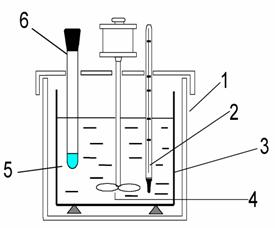
\includegraphics[width=0.25\linewidth]{ris1.jpg}}
\caption{Калориметр с магнитной мешалкой}
\label{ris:image}
\end{figure}

\textbf{Порядок выполнения}

1. Собрать прибор в соответствии с рисунком.

2. Определить постоянную калориметра $K$.

Постоянная калориметра $K$ выражает то количество тепла,  которое необходимо подвести к участвующей в  тепловом  обмене  части калориметра, чтобы повысить его температуру на 1 градус. Для определения постоянной калориметра пользуются кристаллическим хлоридом калия ($KCl$). Необходимо взвесить  на технических весах 2,5 г хлорида калия,  предварительно растертого в ступке, и перенести его в пробирку (3) с пробкой.

Налить в стакан (4) 125 мл воды,  температура которой примерно на 3 $^{o}$C ниже комнатной.
 
Включить мешалку и в течении 20 минут записывать показания термометра с точностью 0.05 град через каждую минуту. На 10-ой минуте, не изменяя температуру,  выталкивают палочкой пробку из пробирки 3 с солью так,  чтобы вся соль высыпалась в воду, и. начиная с 11-ой минуты, вновь каждую минуту делают 10 замеров температуры. Результаты измерений заносят в столбец 3 таблицы (20 строк). 

3. Определить теплоту растворения безводного сульфата меди $Q_{1}$.

Выполнить аналогично п.2 с навеской 2,5 г безводного сульфата меди  ($CuSO_{4}$(безводный)). Результаты измерений заносят в столбец 4 таблицы (20 строк).

4. Определяем теплоту растворения кристаллогидрата $Q_{2}$

Выполнить аналогично п.2 с навеской 2,5 г безводного сульфата меди ($CuSO_{4}\cdot 5H_{2}O$). Результаты измерений заносят в столбец 5 таблицы (20 строк).

\begin{table}[h]
\caption{Экспериментальные данные}
\label{tabular:data1}
\begin{center}
\begin{tabular}{|c|p{4cm}|p{4cm}|p{4cm}|p{4cm}|}
\hline
\No & Время от начала опыта, мин & Навеска $KCl$, $^{o}$C & Навеска $CuSO_{4}(\textrm{безвод.})$, $^{o}$C & Навеска $CuSO_{4}\cdot 5H_{2}O (\textrm{безвод.})$, $^{o}$C\\
\hline
1 & 2 & 3 & 4 & 5 \\
\hline
1 & & & & \\
\hline
 & & & & \\
\hline
20 & & & & \\
\hline
\end{tabular}
\end{center}
\end{table}
\textbf{Обработка экспериментальных данных}

В ходе опыта происходит теплообмен с  окружающей  средой,  т.к. температура воды отличается от комнатной температуры и имеет место выравнивание температур. Поэтому, определить  точную величину изменения температуры ($\Delta t$) при растворении соли по данным, полученным в результате опыта, можно только графическим методом.  График строят в координатах температура --- время.  После нанесения на график всех экспериментально полученных точек, большее число их соединяют прямыми, которые продолжают их до пересечения с перпендикуляром,  восстановленным в 10-ю минуту.  Отрезок, отсекаемый на перпендикуляре, соответствует изменению температуры ($\Delta t$).

Постоянную калориметра вычислить по уравнению:
$$K=\frac{mQ}{M\Delta t}$$

где $m=2,5$г - масса $KCl$; $M$ - молярная масса $KCl$, (г/моль); $Q=18,826$ кДж/моль - молярная  теплота растворения для  $KCl$;

Молярную теплоту растворения безводного сульфата меди ($Q_{1}$) и молярную теплоту растворения кристаллогидрата ($Q_{2}$) вычислить по уравнению:
$$Q_{1}=\frac{K\Delta t_{1}M_{1}}{m_{1}}$$
$$Q_{2}=\frac{K\Delta t_{2}M_{2}}{m_{2}}$$
где $m_{1}=m_{2}=2,5$г - масса навесок соли; $M_{1}$, $M_{2}$ - молярная масса соли, (г/моль);

Вычислить теплоту гидратации ($Q_{3}$) при помощи закона Гесса.
$$CuSO_{4}+5H_{2}O=CuSO_{4}\cdot 5H_{2}O+Q_{3} $$
$$CuSO_{4}=CuSO_{4}(aq)+Q_{1} $$
$$CuSO_{4}\cdot 5H_{2}O= CuSO_{4}(aq)+5H_{2}O+Q_{2}$$
\textbf{Контрольные вопросы}
\begin{enumerate}
\item Что такое тепловой эффект химической реакции?
\item Дайте формулировку закона Гесса.
\item Что  называется  теплотой  (энтропией) образования,  теплотой сгорания? При каких условиях они считаются стандартными?
\item Как по теплоте образования и теплоте сгорания вычислить тепловой эффект реакции?
\item Что понимается под теплотой растворения, теплотой гидратации?
\item Из каких тепловых эффектов складывается  теплота  растворения твёрдого вещества?
\item Что учитывает постоянная калориметра и как её определить?
\item Как определить изменение температуры при растворении?
\end{enumerate}

\newpage
\section{Лабораторная работа 2 }
\textbf{Тема:}Определение коэффициента распределения

\textbf{Цель работы:}Определить коэффициент распределения йода между водой и органическим растворителем -- толуолом.

\textbf{Оборудование и реактивы:} аппарат для встряхивания, бюретка, 4 колбы, с притёртыми пробками на 200 мл, пипетка на 5 мл, мерный цилиндр на 50 мл, раствор йода в толуоле (концентрации: 5, 10, 20 г/л), раствор тиосульфата натрия (концентрация: 0,025 Н).

\textbf{Теория}

Изучение распределения  вещества между двумя несмешивающимися растворителями представляет большой интерес,  так как может  дать ценные сведения, необходимые для проведения экстрагирования, а так же указать на наличие диссоциации,  ассоциации или других химических  реакций  растворенного  вещества в растворе.  Если в систему, состоящую из двух несмешивающихся жидкостей,  ввести небольшое количество вещества,  растворимого в этих жидкостях,  то после установления равновесия, оно распределится между обоими жидкими слоями в определенном, постоянном при данной температуре соотношении.

Экстракцией называют извлечение из многокомпонентного 
раствора одного или нескольких компонентов с помощью растворителя, обладающего избирательной способностью растворять только подлежащий
экстратированию компонент . При помощи экстракции происходит извлечение необходимых веществ: сахара из свёклы, растительного масла из семечек, в формации для алкалоидов и других физиологически активных веществ.	
На основе закона распределения можно рассчитать эффективность экстракции в зависимости от свойств растворителя и экстратирующего вещества.
Экстракция может быть однократной, когда экстратент добавляется в один приём, и дробной – добавления экстратента производится порциями в несколько приёмов.

\textbf{Порядок выполнения}

1. В 4 Колбы на 200 мл с притёртыми пробками отмерить  пипеткой по 5 мл раствора йода различной концентрации и по 50 мл дистиллированной воды.  Полученные смеси энергично встряхивать в течении 30 минут.

2. Перелить содержимое колб в делительные воронки и поставить на 20 минут до расслоения жидкостей.

3. Отделить водный слой, отобрать пипеткой по $V_{\textrm{пр}}=20$ мл из каждой воронки и  оттитровать  йод  0,025 Н раствором тиосульфата натрия ($C_{\textrm{т}}=0,025$моль/л). Раствор тиосульфата прибавляют до появления бледно-желтой  окраски раствора. Затем добавляют  несколько  капель  раствора крахмала и снова титруют раствором тиосульфата натрия до исчезновения  синего окрашивания раствора.  Светло-синяя окраска раствора, появляющаяся через некоторое время после титрования,  не  учитывается.  Пипетку перед отбором пробы ополаскивают исследуемым раствором.

\textbf{Обработка экспериментальных данных}

1. Рассчитать равновесную концентрацию йода (г/л) в водном растворе по формуле:
$$C_{\textrm{в}}=\frac{C_{\textrm{т}}M_{I}V_{\textrm{т}}}{V_\textrm{пр}}$$
Молярная масса йода равна: $M_{I}=127$г/моль.

2. Рассчитать  равновесную  концентрацию йода в толуоле.  Она определяется из уравнения материального баланса для йода при экстракции.
$$m_{0}=m_{\textrm{в}}+m_{\textrm{орг}}$$
$$C_{0}V_{0}=C_{\textrm{в}}V_{\textrm{в}}+C_{\textrm{орг}}V_{\textrm{орг}}$$
$$C_{\textrm{орг}}=\frac{1}{V_{\textrm{орг}}}(C_{0}V_{0}-C_{\textrm{в}}V_{\textrm{в}})$$
При объеме водной фазы $V_{\textrm{в}}=50$мл, объеме органической фазы, раствора йода в толуоле, ($V_{0}=V_{\textrm{орг}}=5$мл) равновесная концентрация йода в толуоле равна:
$$C_{\textrm{орг}}=C_{0}-10C_{\textrm{в}}$$

3. Рассчитать значение константы распределения по формуле:
$$K=\frac{C_{\textrm{орг}}}{C_{\textrm{в}}}=\frac{C_{0}}{C_{\textrm{в}}}-10$$

Все экспериментальные и расчетные данные  сводим  в  таблицу \ref{tabular:data2}.

\begin{table}[h]
\caption{Экспериментальные и расчетные данные}
\label{tabular:data2}
\begin{center}
\begin{tabular}{|c|p{3cm}|p{3cm}|p{3cm}|p{3cm}|p{3cm}|}
\hline
\No & Исходные концентрации йода в толуоле, $C_{0}$, г/л & Объём пробы для титрования, $V_{\textrm{пр}}$, мл & Объем 0,025 Н $Na_{2}S_{2}O_{3}$ пошедшего на титрование, $V_{\textrm{т}}$, мл & Равновесная концентрация йода в воде, $C_{\textrm{в}}$, г/л & Коэффициент распределения, $K$ \\
\hline
1 & 5 & 20 & & & \\
\hline
2 & 10 & 20 & & & \\
\hline
3 & 20 & 20 & & & \\
\hline
\end{tabular}
\end{center}
\end{table}

\textbf{Контрольные вопросы}
\begin{enumerate}
\item Что называется фазой, компонентом и степенью свободы? 
\item В чем заключается физико-химический метод анализа? 
\item На чем основан термический анализ ?
\item Как изображается состав трехкомпонентной системы по методу Гиббса?
\item В чем заключается процесс экстрагирования,  какова его теоретическая основа?
\item Что такое мольная доля?
\item Что такое химический потенциал?
\item Закон распределения.
\item Правило фаз Гиббса.
\end{enumerate}
\newpage
\section{Лабораторная работа 3 }
\textbf{Тема:}Построение диаграмм состояния трехкомпонентной системы с ограниченной взаимной растворимостью.

\textbf{Цель работы:}Построить диаграмму состояния тройной системы $CH_{3}COOH$ --- $CH_{3}Cl$ --- $H_{2}O$.

\textbf{Оборудование и реактивы:} бюретка, 8 колб, с притёртыми пробками на 200 мл, пипетка на 5 мл, мерный цилиндр на 50 мл, раствор $CH_{3}COOH$, раствор $CH_{3}Cl$.

\textbf{Теория}

Физико-химический анализ  устанавливает  количественную зависимость между составом и каким-нибудь измеренным физическим свойством  системы (температурой кипения,  плавления,  давления пара, электропроводностью и др.) Графическое изображение зависимости какого либо свойства от состава системы или другого фактора равновесии ее (например, давления) называется диаграммой состояния. Диаграммы состояния позволяют сделать выводы о взаимодействиях отдельных веществ в системе,  образования новых  химических  соединений, твердых растворов, их составе и границе существования.

Для разбора диаграмм состояния широко применяется теория равновесия  неоднородных (гетерогенных) систем,  прежде всего -- правило фаз Гиббса.

Ознакомившись с сущностью физико-химического анализа,  его значением,  с понятием фаза,  компонент и степени свободы,  обратите внимание на следующее: фаза не адекватна понятию агрегатного состояния и в однокомпонентных системах в равновесии могут находиться две фазы одного агрегатного состояния.

Число степеней свободы ($C$) определяется числом компонентов ($K$) и фаз ($F$), находящихся  в  равновесной  системе ($C=K+2-F$).

Студентам необходимо  приобрести  навыки  чтения  диаграмм состав-свойство различных бинарных жидких смесей,  диаграмм плавкости и простейших диаграмм трехкомпонентных систем. При выполнении лабораторной работы необходимо научиться определять в любой точке на диаграмме число компонентов и фаз,  состав системы и весовые соотношения компонентов,  уметь находить температуру  начала  и  конца кристаллизации и плавления,  кипения и конденсации. Надо знать, на основании каких экспериментальных данных строятся различные  диаграммы.

В тех случаях, когда система состоит из трех компонентов, пользуются треугольником Гиббса. Принимают, что каждая вершина равностороннего треугольника отвечает 100\% составу одного из  компонентов,  а каждая сторона -- двойной системе из компонентов, указанных в вершинах, которые она соединяет.

\begin{figure}[h]
\center{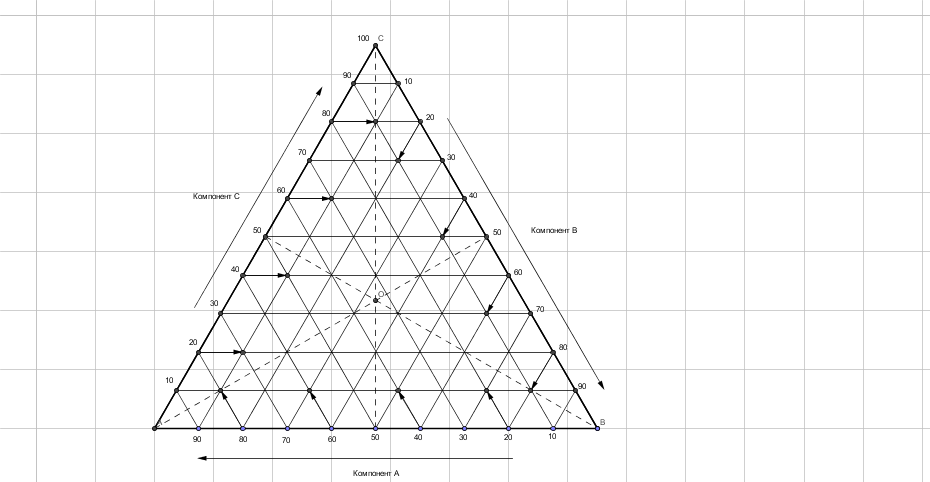
\includegraphics[width=0.5\linewidth]{gibbs.png}}
\caption{Треугольник Гиббса}
\label{ris:image}
\end{figure}

В треугольнике проводят три высоты,  делят каждую высоту на десять равных отрезков и через полученные деления проводят прямые, с помощью которых можно представить любой состав тройной системы.

Чтобы нанести точку, отвечающую составу трехкомпонентной системы, на двух высотах откладывают процентное содержание соот-ветствующих компонентов.  Через полученные точки на высотах проводят прямые,  параллельные сторонам, лежащим против угла, вершина которого отвечает содержанию чистого компонента.  Точка пересечения  прямых будет отвечать искомому составу.

\textbf{Порядок выполнения}

1. В 8  Колб  с  притертыми  пробками наливают по 10 мл бинарных смесей взаимно растворимых друг в друге веществ ($CH_{3}COOH$ --- $CH_{3}Cl$)  в соотношении, указанном в таблице \ref{tabular:data3}.

\begin{table}[h]
\caption{Объемы компонентов бинарных смесей}
\label{tabular:data3}
\begin{center}
\begin{tabular}{|p{6cm}|c|c|c|c|c|c|c|c|}
\hline
\No колбы & 1 & 2 & 3 & 4 & 5 & 6 & 7 & 8 \\
\hline
Объем $CH_{3}COOH$, мл & 2 & 4 & 6 & 7 & 7,5 & 8 & 8,5 & 9 \\
\hline
Объем $CH_{3}Cl$, мл & 8 & 6 & 4 & 3 & 2,5 & 2 & 1,5 & 1 \\
\hline
Объем $H_{2}O$, мл & & & & & & & &  \\
\hline
\end{tabular}
\end{center}
\end{table}

2. Растворы титруют водой до появления мути.  В некоторых опытах для этого достаточно одной-двух капель воды.  Результаты занося  в таблицу \ref{tabular:data3}.

\textbf{Обработка экспериментальных данных}

1. Для расчёта количеств веществ компонентов пользуются формулой:
$$n=\frac{V \cdot \rho}{M}$$
где $n$ - количество вещества, моль;

$V$ - объем вещества, мл;

$\rho$ - плотность (приведена в таблице \ref{tabular:data4});

$M$ - Молярная масса, г/моль.

Рассчитайте молярные массы компонентов и занесите результат в таблицу \ref{tabular:data4}.

\begin{table}[h]
\caption{Данные для рассчета}
\label{tabular:data4}
\begin{center}
\begin{tabular}{|p{5cm}|p{5cm}|p{5cm}|}
\hline
Вещество & Плотность, г/мл & Молярная масса, г/моль\\
\hline
$CH_{3}COOH$ & 1,06 & \\
\hline
$CH_{3}Cl$ & 1,5 &  \\
\hline
$H_{2}O$ & 1,0 &  \\
\hline
\end{tabular}
\end{center}
\end{table}

2. Рассчитать количество вещества компонентов системы, результат занести в таблицу \ref{tabular:data5}.

\begin{table}[h]
\caption{Состав бинарных смесей, моль}
\label{tabular:data5}
\begin{center}
\begin{tabular}{|p{8cm}|c|c|c|c|c|c|c|c|}
\hline
\No колбы & 1 & 2 & 3 & 4 & 5 & 6 & 7 & 8 \\
\hline
Количество вещества $CH_{3}COOH$, моль & & & & & & & & \\
\hline
Количество вещества $CH_{3}Cl$, моль & & & & & & & & \\
\hline
Количество вещества $H_{2}O$, моль & & & & & & & &  \\
\hline
Всего, моль & & & & & & & &  \\
\hline
\end{tabular}
\end{center}
\end{table}

3. Рассчитывают состав системы в мольных долях, отвечающий началу расслоения (появления мути).
Мольной долей компонента ($x$) считают  отношение  числа молей данного компонента к сумме молей всех компонентов раствора. Например, мольную долю компонента $A$ вычисляют по уравнению:
$$x=\frac{n_{A}}{n_{A}+n_{B}+n_{C}}$$
Мольные доли других компонентов вычисляют по подобным уравнениям. Результаты рассчетов занести в таблицу \ref{tabular:data5}. Сумма мольных долей всех компонентов должна быть равна $1$.

4. Полученные данные наносят на треугольную диаграмму.  Соединив точки, получают плавную кривую,  по одну сторону которой находится гетерогенная область, по другую -- гомогенная.

\begin{table}[h]
\caption{Состав бинарных смесей, мольные \%}
\label{tabular:data3}
\begin{center}
\begin{tabular}{|p{8cm}|c|c|c|c|c|c|c|c|}
\hline
\No колбы & 1 & 2 & 3 & 4 & 5 & 6 & 7 & 8 \\
\hline
Мольная доля $CH_{3}COOH$, \% & & & & & & & & \\
\hline
Мольная доля $CH_{3}Cl$, \% & & & & & & & & \\
\hline
Мольная доля $H_{2}O$, \% & & & & & & & &  \\
\hline
Всего & & & & & & & &  \\
\hline
\end{tabular}
\end{center}
\end{table}

\textbf{Контрольные вопросы}
\begin{enumerate}
\item Что называется фазой, компонентом и степенью свободы? 
\item В чем заключается физико-химический метод анализа? 
\item На чем основан термический анализ ?
\item Как изображается состав трехкомпонентной системы по методу Гиббса?
\item В чем заключается процесс экстрагирования,  какова его теоретическая основа?
\item Что такое мольная доля?
\item Что такое химический потенциал?
\item Закон распределения.
\item Правило фаз Гиббса.
\end{enumerate}
\chapter{Химическая кинетика}
\newpage
\section{Лабораторная работа 4 }
\textbf{Тема:}Определение энергии активации и порядка реакции разложения пероксида водорода.

\textbf{Цель работы:}газометрическим методом определить порядок и энергию активации реакции разложении пероксида водорода ($H_{2}O_{2}$).

\textbf{Оборудование и реактивы:} установка для изучения разложения $H_{2}O_{2}$, термостат, термометр, пробирки на 20 - 25 мл., раствор $CuSO_{4}$ (1 Н), раствор пероксида водорода (4\%), $MnO_{2}$, вода.

\textbf{Теория}
\textit{\textbf{1. Определение порядка реакции.}}

Пероксид водорода в водных растворах самопроизвольно разлагается по уравнению:
$$H_{2}O_{2}\rightarrow H_{2}O+0.5O_{2}\uparrow$$
В присутствии некоторых веществ разложение пероксида водорода значительно ускоряется. В данной работе катализаторами могут быть сульфат меди или оксид марганца(IV).

Поскольку и $CuSO_{4}$, и $H_{2}O_{2}$ находятся в водном растворе (одна фаза), эта реакция является гомогенной каталитической реакцией. Оксид марганца (IV) используется в виде порошка (две фазы), тогда реакция является гетерогенной каталитической.

$$r=kC^{x},$$
где $C$ -- концентрация пероксида водорода, моль/л;

$k$ -- кинетическая константа реакции;

$x$ -- порядок реакции.

Для определения величин порядка реакции и кинетической константы построим график в координатах $ln(r)$ --- $ln(C)$. 
$$ln(r)=ln(k)+x\cdot ln(C)$$
Тогда порядок реакции определится как тангенс угла наклона прямой, а $ln(k)$ --- по отрезку, отсекаемому прямой на вертикальной оси.
Концентрация пероксида водорода может быть расчитана по формуле:
$$C=\frac{n_{01}-X}{V}=C_{0}-\frac{X}{V_{1}},$$
где $n_{01}$ -- начальное количество пероксида водорода,моль;

$X$ -- количество прореагировавшего пероксида водорода, моль;

$C_{0}$ -- начальная концентрация пероксида водорода, моль/л.

$V_{1}$ -- объем реакционной смеси, л.

Величину $X$ определим из реакции через объем выделившегося кислорода. Последний свяжем с количеством вещества через уравнение Менделеева-Клапейрона.
$$PV=n_{3}RT,$$
$$X=2n_{3}=\frac{2PV}{RT}=\frac{2\cdot 101325\cdot V}{8,31\cdot 298}=81,83V$$
$P$ -- давление, Па;

$V$ -- объем выделившегося кислорода, м~$^{3}$;

$n_{3}$ -- количество выделившегося кислорода, моль;

$R$ -- газовая постоянная;

$T$ -- температура, К.

Тогда: 
$$C=C_{0}-0,082\cdot\frac{V}{V_{1}}$$
Среднюю скорость реакции расчитаем по формуле:
$$r=\frac{\Delta C}{\Delta\tau}=\frac{0,082V}{V_{1}\cdot\Delta\tau}$$
где $\Delta\tau$ -- интервал времени, мин.

Величину начальной молярной концентрации пероксида водорода определить по таблице 1. Объемы в формулах (1), (2) брать в миллилитрах.

\begin{table}[h]
\caption{Плотности растворов пероксида водорода ($M=34,01$г/Моль) при 18~$^{o}$~C}
\label{tabular:data22_1}
\begin{center}
\begin{tabular}{|p{5cm}|p{5cm}|}
\hline
Массовая доля, \% & Плотность, г/мл \\
\hline
1 & 1,0022\\
\hline
2 & 1,0058\\
\hline
4 & 1,0131\\
\hline
6 & 1,0204\\
\hline
8 & 1,0277\\
\hline
10 & 1,0351\\
\hline
\end{tabular}
\end{center}
\end{table}

\textit{\textbf{2. Определение порядка реакции по уравнениям кинетических констант}}

Величину порядка реакции и кинетической константы можно определить по известным уравнениям для кинетических констант реакции порядка 0, 1, 2, 3, ...

Для этого по уравнениям из таблицы \ref{tabular:data22_2} для кинетических констант реакций различных порядков рассчитывают величины констант для каждого момента времени по экспериментальным данным. Если реакция имеет целочисленный порядок, то соответствующая расчетная величина константы будет сохранять постоянство на всем интервале измерения.
\begin{table}[h!]
\caption{Кинетические характеристики реакций 1-го, 2-го и 3-го порядков}
\label{tabular:data22_2}
\begin{center}
\begin{tabular}{|>{\centering\arraybackslash}p{0.1\linewidth}|>{\centering\arraybackslash}p{0.15\linewidth}|>{\centering\arraybackslash}p{0.25\linewidth}|>{\centering\arraybackslash}p{0.2\linewidth}|>{\centering\arraybackslash}p{0.15\linewidth}|}
\hline 
Порядок реакции (общий) &
Дифферен-\- циальное уравнение $r=r(C,T)$, размерность кинетической константы $[k]$ &
Интегральное уравнение, $C=C(\tau,T)$ выражение для кинетической константы $k$&
Степень превращения $\alpha=\frac{C_{0}-C}{C_{0}}$&
Время полупревращения, $\tau_{0,5}$ ($\alpha=0,5$, $C=0,5C_{0}$)
\\ 
\hline 
0 & $$-\frac{dC}{d\tau}=k$$ 
$$[k]=\frac{\textsc{моль}}{\textsc{м}^{3}\textsc{с}}$$& 
$$C=C_{0}-k\tau$$ 
$$k=\frac{C_{0}-C}{\tau}$$ &
$$\alpha=\frac{k\tau}{C_{0}}$$ & 
$$\tau_{0,5}=\frac{C_{0}}{2k}$$\\ 
\hline 
1 &  $$-\frac{dC}{d\tau}=kC$$ 
$$[k]=\textsc{с}^{-1}$$&
$$ln(C)=ln(C_{0})-k\tau$$
$$k=\frac{1}{\tau}\cdot ln\left(\frac{C_{0}}{C}\right)$$&
$$\alpha=1-e^{-k\tau}$$ &
$$\tau_{0,5}=\frac{ln(2)}{2k}$$\\ 
\hline 
2 &  $$-\frac{dC}{d\tau}=kC^{2}$$ 
$$[k]=\frac{\textsc{м}^{3}}{\textsc{моль}\textsc{с}}$$&
$$\frac{1}{C}=\frac{1}{C_{0}}+k\tau$$
$$k=\frac{1}{\tau}\cdot\left(\frac{1}{C}-\frac{1}{C_{0}}\right)$$&
$$\alpha=\frac{k\tau C_{0}}{k\tau C_{0}+1}$$&
$$\tau_{0,5}=\frac{1}{kC_{0}}$$\\ 
\hline 
3 & $$-\frac{dC}{d\tau}=kC^{3}$$ 
$$[k]=\frac{(\textsc{м}^{3})^{2}}{\textsc{моль}^{2}\textsc{с}}$$&
$$\frac{1}{C^{2}}=\frac{1}{C_{0}^{2}}+2k\tau$$
$$k=\frac{1}{2\tau}\cdot\left(\frac{1}{C^{2}}-\frac{1}{C_{0}^{2}}\right)$$&
$$k=\frac{\alpha(2-\alpha)}{2\tau C_{0}^{2}(1-\alpha)^{2}}$$&
$$\tau_{0,5}=\frac{3}{2kC_{0}}$$\\ 
\hline 
\end{tabular} 
\end{center}
\end{table}

\textit{\textbf{3. Определение энергии активации.}}

Зависимость константы скорости от температуры выражается уравнением Аррениуса:
$$ln(k)=ln(k_{0})-\frac{E}{R}\cdot\frac{1}{T},$$
где: $E$ -- энергия активации;

В координатах $ln(k)$ --- $\frac{1}{T}$ экспериментальные данные должны лежать на прямой. Её тангенс угла наклона $tg(\phi)$ находят из графика, а затем, вычисляют Е:
$$E=R\cdot tg(\phi)$$
Возможно также применение аналитического метода. Решаем систему уравнений Аррениуса относительно $E$ и $k_{0}$.
$$
\begin{cases}
ln(k_{1})= ln(k_{0})-\frac{E}{R}\cdot\frac{1}{T_{1}}\\
ln(k_{2})= ln(k_{0})-\frac{E}{R}\cdot\frac{1}{T_{2}}
\end{cases}
$$

Решение:
$$E=\frac{RT_{1}T_{2}}{T_{1}-T_{2}}ln\left(\frac{k_{1}}{k_{2}}\right)$$
$$k_{0}=\frac{T_{1}ln(k_{1})-T_{2}ln(k_{2})}{T_{1}-T_{2}}$$

\textbf{Порядок выполнения}
Наблюдение за ходом реакции и определение её скорости ведется путём измерения объёма выделившегося кислорода (газометрический метод). Измерения проводят через определенные промежутки времени от начала реакции. Прибор для работы (Рис. \ref{ris:image22_1}.) состоит из реакционной пробирки 1, бюретки 2 и уравнительного сосуда 3, соединённого резиновым шлангом с нижней частью измерительной бюретки.
Пробирка с реакционной смесью помещается в водяной термостат 4.

\begin{figure}[h]
\center{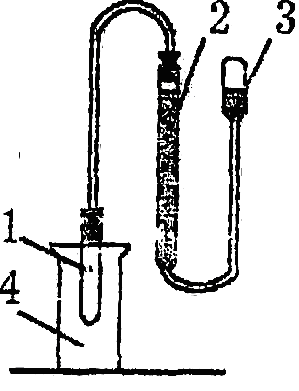
\includegraphics[width=0.25\linewidth]{volume.png}}
\caption{Схема экспериментальной установки}
\label{ris:image22_1}
\end{figure}
\underline{При использовании в качестве катализатора $CuSO_{4}$:}

В реакционную пробирку 1 наливают 10 мл раствора $CuSO_{4}$ (1 Н) и 10 мл дистиллированной воды; пробирку помещают в термостат. Передвигая уравнительный сосуд вверх и вниз, устанавливают уровень жидкости в бюретке на нуле. После 10-ти минутного термостатирования в смесь вливают 5 мл 4\% раствора $H_{2}O_{2}$, тщательно перемешивают, записывают время опыта и температуру. Общий объем жидкости 25 мл.

\underline{При использовании в качестве катализатора $MnO_{2}$:}

В реакционную пробирку 1 засыпают примерно 1 г $MnO_{2}$, заливают 10 мл дистиллированной воды; пробирку помещают в термостат. Передвигая уравнительный сосуд вверх и вниз, устанавливают уровень жидкости в бюретке на нуле. После 10-ти минутного термостатирования в смесь вливают 5 мл 4\% раствора $H_{2}O_{2}$, тщательно перемешивают, записывают время опыта и температуру. 

Выделяющийся кислород будет вытеснен из бюретки. Через определенные промежутки времени отсчитывают объем выделившегося кислорода. Реакция считается законченной, если уровень жидкости в бюретке перестанет опускаться. Результаты опыта записывают в таблицу \ref{tabular:data22_3}.

Первый опыт проводят при комнатной температуре. Затем повторяют опыт ещё 1 – 2 раза при других температурах. Таблица \ref{tabular:data22_3} заполняется отдельно для результатов при каждой температуре для каждого катализатора.

Рекомендуемые интервалы между отсчётами: при температуре термостата 20-25~$^{o}$~С --- интервал 5 минут; при температуре 30-40~$^{o}$~С --- 3 минуты. 

\begin{table}[h]
\caption{Экспериментальные данные}
\label{tabular:data22_3}
\begin{center}
\begin{tabular}{|p{0.15\linewidth}|p{0.4\linewidth}|p{0.4\linewidth}|}
\hline
\No\ измерения & Время от начала опыта, $\tau$, мин & Объём кислорода $V$, мл \\
\hline
& & \\
\hline
\end{tabular}
\end{center}
\end{table}

\textbf{Обработка экспериментальных данных}

\textit{\textbf{1. Определение порядка реакции.}}

Расчеты в таблицах \ref{tabular:data22_4}, \ref{tabular:data22_5} выполняются для всех серий измерений, для которых получены данные в таблице \ref{tabular:data22_3} (для всех катализаторов при различных температурах), при которых проводился эксперимент. Для каждой температуры следует заполнить указанные таблицы.

Заполнить таблицу \ref{tabular:data22_4}. Расчет выполняется по формулам (1), (2).
\begin{table}[h]
\caption{Результаты расчетов для определения порядка реакции дифференциальным методом}
\label{tabular:data22_4}
\begin{center}
\begin{tabular}{|p{0.15\linewidth}|p{0.15\linewidth}|p{0.15\linewidth}|p{0.22\linewidth}|p{0.22\linewidth}|}
\hline
\No\ измерения& $\tau$, мин & $C_{H_{2}O_{2}}$, моль/л & $ln(r)$ & $ln(C)$ \\
\hline 
 & & & & \\
\hline
\end{tabular}
\end{center}
\end{table}

Заполнить таблицу \ref{tabular:data22_5}. Расчет выполняется по формулам для кинетических констант 0-го, 1-го, 2-го, 3-го порядков из таблицы \ref{tabular:data22_2}.
\begin{table}[h]
\caption{Результаты расчета для определения порядка реакции интегральным методом}
\label{tabular:data22_5}
\begin{center}
\begin{tabular}{|p{0.15\linewidth}|p{0.15\linewidth}|p{0.15\linewidth}|p{0.1\linewidth}|p{0.1\linewidth}|p{0.1\linewidth}|p{0.1\linewidth}|}
\hline
\No\ измерения& $\tau$, мин & $C_{H_{2}O_{2}}$, моль/л & $k_{0}$ & $k_{1}$ & $k_{2}$ & $k_{3}$ \\
\hline 
 & & & & & & \\
\hline
\end{tabular}
\end{center}
\end{table}

\textit{\textbf{2. Определение энергии активации.}}

В случае использования графического метода заполняют таблицу \ref{tabular:data22_6} и строят график в координатах $ln(k)$---$\frac{1}{T}$.

Для выполнения расчета по уравнению Аррениуса можно воспользоваться формулами (3).

\begin{table}[h]
\caption{Результаты расчетов для определения параметров уравнения Аррениуса}
\label{tabular:data22_6}
\begin{center}
\begin{tabular}{|p{0.22\linewidth}|p{0.22\linewidth}|p{0.22\linewidth}|p{0.22\linewidth}|}
\hline
 $$T,$$ K& $$k$$ & $$ln(k)$$ & $$\frac{1}{T}$$ \\
\hline 
 & & & \\
\hline
\end{tabular}
\end{center}
\end{table}

\textbf{Контрольные вопросы}
\begin{enumerate}
\item Что называют скоростью химической реакции?
\item Что такое средняя и истинная скорость?
\item Какие факторы влияют на скорость химических реакций?
\item Сформулируйте закон действующий масс.
\item Что такое константа скорости химической реакции? 
\item Как зависит скорость химической реакции от температуры?
\item Что такое энергия активации? Какова зависимость между скоростью реакции и энергией активации?
\item Что такое молекулярность химической реакции?
\item Что такое порядок химической реакции?
\item В каких случаях молекулярность и порядок химической реакции не совпадают?
\item Какой вид имеет кинетическое уравнение химической реакции 1-го и 2-го и любого другого порядка?
\item На основании каких данных рассчитываются энергии активации?
\item Что называют катализом и катализатором? Какое влияние оказывает катализатор на энергию активации реакции?
\item Что такое гомогенный катализ? Механизм гомогенного катализа?
\item Гетерогенный катализ? Стадии гетерогенного катализа?
\item Методы ускорения гетерогенного катализа?
\end{enumerate}


\chapter{Электрохимия}
\newpage
\section{Лабораторная работа 5 }
\textbf{Тема:}Определение константы диссоциации слабого электролита.

\textbf{Цель работы:} Определение константы диссоциации слабого электролита методом измерения электропроводности раствора. Изучение влияния концентрации электролита на величину константы диссоциации.

\textbf{Оборудование и реактивы:} кондуктометр, мерный цилиндр на 100 мл, мерные колбы на 100 мл, 1 М раствор $CH_{3}COOH$, стакан, вода.

\textbf{Теория}
\textit{\textbf{1. Проводники и диэлектрики}}
Способность вещества  проводить  электрический  ток  называется электропроводностью. Электропроводность является величиной, обратной электрическому сопротивлению (способности вещества препятствовать прохождению электрического тока).  Характер и количество частиц носителей зарядов (ионов,  электронов) зависит от природы вещества,  его агрегатного состояния, температуры и других факторов, а электрическое поле определяется разностью электрических потенциалов между полюсами и способностью вещества к ионизации.  Вещества различают по проводимости электрического тока.  Строго говоря, все вещества способны проводить электрический ток,  но в практических целях их делят на проводники и непроводники (диэлектрики или  изоляторы),  так как первые обладают в миллионы раз большей проводимостью,  чем вторые. В зависимости от природы частиц носителей зарядов  различают два рода проводников.  К проводникам первого рода относят графит, металлы в твердом и расплавленном состоянии, когда носителями зарядов являются электроны.
К проводникам второго рода относят растворы электролитов,  газы при достаточной степени ионизации и растворы некоторых солей, когда носителями зарядов являются ионы, перемещение которых определяет электро-проводность. Непроводниками считают слюду, фарфор, химически чистую воду,  кристаллы солей, многие низко- и высокомолекулярные  органические соединения и другие.  Некоторые непроводники, приобретающие при изменении внешних условий (температурное, световое, радиационное или другое воздействие) проводимость, называются полупроводниками.  Проводимость в этих веществах возникает, потому что  электроны  переходят в свободное состояние за счет увеличения интенсивности теплового движения частиц тока или за счет положения энергии.  Такими свойствами обладают элементы:  $B$, $C$, $Si$, $Ge$, $Te$, $P$, $S$, $Se$; сплавы: $Mg_{3}Sb_{2}$, $ZnSb$, $InSb$ и др.; оксиды: $Al_{2}O_{3}$, $Cu_{2}O$ и др.; сульфиды : $Cu_{2}S$, $Ag_{2}S$, $ZnS$ и др.; селениды и множество других более сложных соединений.

\textit{\textbf{2. Электропроводимость растворов электролитов}}

Электролиты --- химические соединения,  которые в  растворе  полностью или частично диссоциируют на ионы. Различают сильные и слабые электролиты. Силу электролита характеризуют величиной, названной Арреииусом степенью электрической диссоциации $\alpha$. Под степенью диссоциации понимают соотношение числа молекул, распавшихся на ионы, к общему числу молекул в растворе. Сильные электролиты практически полностью диссоциированы на ионы ($\alpha\approx 1$). К ним относятся многие неорганические соли и кислоты. Для слабых электролитов степень диссоциации очень мала ($\alpha<1$).
Классическая теория  электролитической диссоциации,  созданная Аррениусом (1887),  применена только к разбавленным растворам слабых электролитов. Эта теория исходит из представления, что в растворе электролита существует динамическое равновесие между недиссоциированными молекулами и ионами. Например для уксусной кислоты:
$$CH_{3}COOH\leftrightarrows H^{+}+CH_{3}COO^{-}$$
Количественно это  равновесие можно охарактеризовать константой равновесия, она же константа диссоциации:
$$K=\frac{C_{CH_{3}COO^{-}}\cdot C_{H^{+}}}{C_{CH_{3}COOH}}$$
Константа диссоциации зависит от природы растворенного вещества и растворителя, а так же от температуры.
Степень диссоциации ($\alpha$) и константа диссоциации связаны уравнением Оствальда.
$$K=\frac{\alpha^{2}\cdot C}{1-\alpha}$$
Константа диссоциации  может  быть  определена экспериментально различными методами.  Наиболее распространенным  методом  является метод измерения электрической проводимости растворов.

Под электрической  проводимостью $L$ (электропроводимостью) понимается величина, обратная сопротивлению ($R$): $L = R^{-1}$.

В системе СИ единицей электрической проводимости является сименс (См),  равный  электрической  проводимости проводника, имеющего сопротивление 1 Ом, т.е. [См] = [1/Ом].

Электропроводимость растворов зависит от концентрации ионов, от природы  электролита  и растворителя,  от скорости движения ионов, вязкости и диэлектрической постоянной растворителя.

Различают удельную  и  эквивалентную  проводимость  растворов электролитов.

Удельной электрической проводимостью $\kappa$ ($[\kappa]=$См/см) называют электрическую проводимость раствора,  заключенного между  электродами, площадью по 1 см$^{2}$ и расстоянием 1 см между ними.

Эквивалентная электрическая проводимость $\lambda$ ($[\lambda]=$См см$^{2}$ экв$^{-1}$) равна электрической проводимости  раствора, содержащего  один  эквивалент рас-творенного вещества между электронами, расстояние между которыми равно 1 см.

Площадь электрода определяется объемом раствора. Чем больше разбавление, тем больше  объем  раствора,  и  тем  больше  площадь электродов. Эквивалентная  проводимость и удельная электропроводимость связаны  между  собой  соотношением:
$$\lambda=\frac{\kappa\cdot 1000}{C},$$
где $C$ -- концентрация (экв/л);

Концентрированные растворы  электролитов имеют малое значение электронной проводимости. С разбавлением раствора эта величина увеличивается и при бесконечном разбавлении достигает максимального и постоянного для каждого электролита значения.  Эта  величина обозначается  и называется эквивалентной электрической проводимостью при бесконечном разбавлении. В соответствии с законом Кольреуша может быть вычислена :
$$\lambda_{0}=u_{+}^{0}+u_{-}^{0},$$
где $u_{+}^{0}$ и $u_{-}^{0}$ -- подвижности катионов и анионов (находят по таблице \ref{tabular:data31_1}).

Эквивалентная электрическая проводимость может быть использована для определения степени и константы  электрической диссоциации. По уравне-нию Аррениуса:
$$\alpha=\frac{\lambda}{\lambda_{0}}$$
Тогда:
$$K=\frac{\lambda^{2}C}{\lambda_{0}(\lambda_{0}-\lambda)}$$

\begin{longtable}[h]{|c|c|c|c|}
\caption{Таблица Предельные подвижности $u^{0}_{i}$ некоторых ионов в водном растворе при 25$^{o}$C [Ом$^{-1}$см$^{2}$/г-экв]\label{tabular:data31_1}}\\
\hline
Катионы	 & $u^{0}_{i}$ & Анионы &$u^{0}_{i}$ \\
\hline\endfirsthead
\endhead
$H^{+}$ & 349,8 & $OH^{-}$ & 198,3 \\
\hline 
$Li^{+}$ & 36,68 & $F^{-}$ & 55,4 \\
\hline 
$Na^{+}$ & 50,10 & $Cl^{-}$ & 76,35 \\
\hline 
$K^{+}$ & 73,50 & $Br^{-}$ & 78,14 \\
\hline 
$Rb^{+}$ & 77,81 & $I^{-}$ & 78,84 \\
\hline 
$Ag^{+}$ & 61,90 & $ClO_{3}^{-}$ & 64,6 \\
\hline 
$NH_{4}^{+}$ & 73,55 & $ClO_{4}^{-}$ & 67,36 \\
\hline 
$N(CH3)_{4}^{+}$ & 44,92 & $BrO_{3}^{-}$ & 55,74 \\
\hline 
$1/2 Mg^{2+}$ & 53,05 & $CN^{-}$ & 78 \\
\hline 
$1/2 Ca^{2+}$ & 59,50 & $NO_{3}^{-}$ & 71,46 \\
\hline 
$1/2 Ba^{2+}$ & 63,63 & $CH_{3}COO^{-}$ & 40,90 \\
\hline 
$1/2 Mg^{2+}$ & 56,6 & $C_{6}H_{5}COO^{-}$ & 35,8 \\
\hline 
$1/2 Cd^{2+}$ & 54 & $H_{2}PO_{4}^{-}$ & 36 \\
\hline 
$1/3 Al^{3+}$ & 63 & $1/2 SO_{4}^{2-}$ & 80,02 \\
\hline 
$1/3 La^{3+}$ & 69,7 & $1/2 S_{2}O_{6}^{2-}$ & 93 \\
\hline 
\end{longtable}

\textbf{Порядок выполнения}
Пипеткой в ячейку наливают 100 мл исследуемого раствора слабого электролита (электролит берут по  указанию  преподавателя)  и измеряют три раза его сопротивление,  перемешивая перед каждым измерением. Далее раствор разбавляют два раза,  для чего из  стакана (ячейки) отбирают пипеткой 50 мл исследуемого раствора,  переносят его в чистый стакан и добавляют туда этой же пипеткой 50 мл дистиллированной воды. Разбавленный раствор заливают в ячейку и измеряют электропроводность.
Далее измеряют  удельную электропроводность  растворов,  разбавленных соответственно в 4,  8, 16 и 32 раза (т.е. делают ещё 4 последовательных двойных разбавления  как описано  выше).  Результаты записывают в таблицу \ref{tabular:data31_2}. 
После окончания  работы  с электродами их тщательно промывают дистиллированной водой.

\begin{table}[h]
\caption{Экспериментальные данные}
\label{tabular:data31_2}
\begin{center}
\begin{tabular}{|p{0.1\linewidth}|p{0.2\linewidth}|p{0.2\linewidth}|p{0.2\linewidth}|p{0.15\linewidth}|}
\hline
\No\ измерения & Концентрация электролита, $C$, моль-экв/л & Удельная электропроводность $\kappa$, См/см & Эквивалентная электропроводность $\lambda$, моль-экв/л & Константа диссоциации $K$\\
\hline
& & & & \\
\hline
\end{tabular}
\end{center}
\end{table}

\textbf{Обработка экспериментальных данных}
Измерив удельную электропроводность всех  растворов,  рассчитывают для них значения нормальной концентрации $C$, эквивалентной электропроводности, $\lambda$, и константу диссоциации $K$. Результаты расчетов вносят в таблицу \ref{tabular:data31_2}.

Нормальную концентрацию рассчитывают по  исходному  значению  её учетом двукратных последовательных разбавлений  в $a$ раз ($a=0,5$).
$$C_{0}=\frac{n_{0}}{V}$$
При разбавлении:
$$n_{1}=C_{0}\cdot V\cdot a$$
Новая концентрация разбавленного в $a$ раз раствора равна:
$$C_{1}=\frac{n_{1}}{V}=C_{0}\cdot a$$
или:
$$C_{i}=C_{0}\cdot a^{i}$$

Эквивалентную электропроводность расчитывают по формуле:
$$\lambda=\frac{\kappa\cdot 1000}{C}$$

Константу диссоциации для одноосновных кислот рассчитывают по формуле:
$$K=\frac{\lambda^{2}C}{\lambda_{0}(\lambda_{0}-\lambda)},$$
где $\lambda_{0}$ -- эквитвалентная электропроводность предельно разбавленного раствора, определяемая по закону Кольрауша:
$$\lambda_{0}=u_{+}^{0}+u_{-}^{0},$$
где $u_{+}^{0}$ и $u_{-}^{0}$ -- подвижности катионов и анионов (находят по таблице \ref{tabular:data31_1}).

Вычислив значение  $K$  для  различных  концентраций слабого электролита, сделать вывод о влиянии концентрации электролита на величину константы диссоциации.

\textbf{Контрольные вопросы}
\begin{enumerate}
\item Что такое электролитическая диссоциация? Виды диссоциации. 
\item Степень диссоциации, константа диссоциации.
\item Подвижность ионов. Закон Кольрауша. Числа переноса ионов.
\item Что такое изотонический коэффициент? Его влияние на законы идеальных растворов.
\item Что такое слабые и сильные электролиты?
\item Закон Оствальда. Вывод уравнения для одноосновных кислот. Записать уравнения закона Оствальда для данного электролита через степень диссоциации и через эквивалентную электропроводность.
\item Закон Оствальда. Вывод уравнения для двухосновных кислот. Записать уравнения закона Оствальда для данного электролита через степень диссоциации и через эквивалентную электропроводность.
\item Для каких электролитов применяют законы разведения?
\item Что такое удельная эквивалентная электропроводимость?
\item От чего зависит электропроводность растворов? 
\item Как, исходя из теории электролитической диссоциации и теории сильных  электролитов,  объяснить  зависимость $K$ и $\lambda$ от разбавления?
\end{enumerate}


\newpage
\section{Лабораторная работа 6 }
\textbf{Тема:}Определение коэффициента электропроводности сильного электролита.

\textbf{Цель работы:} Изучение влияния разбавления на электропроводность сильных электролитов. Определение коэффициента электропроводности сильного электролита методом измерения электропроводности раствора. Графическое построение зависимостей удельной электропроводности от концентрации и эквивалентной электропроводимости от разбавления. 


\textbf{Оборудование и реактивы:} кондуктометр, мерный цилиндр на 100 мл, мерные колбы на 100 мл, раствор $KCl$, раствор $NaCl$, стакан, вода.

\textbf{Теория}
\textit{\textbf{1. Электропроводность сильных электролитов }}
В водных растворах сильные электролиты находятся преимущественно в  виде  ионов.  При разбавлении эквивалентная проводимость растворов увеличивается,  достигая предельного  значения $\lambda_{0}$. Удельная электропроводность тоже растет, но кривая зависимости ее от разбавления проходит через максимум.  Влияние разбавления на электропроводимость растворов сильных электролитов объясняется ослаблением межионного  взаимодействия  при уменьшении  концентрации электролита. Электрическое взаимодействие ионов влияет на характер их распределения  в  растворах,  особенно   в   концентрированных. Вследствии этого  число  ионов в растворе становится как бы меньше числа, соответствующего их концентрации при полной диссоциации,  в связи с  этим  вводится понятие коэффициента электропроводности $f$:
$$f=\frac{\lambda}{\lambda_{0}}$$
При разбавлении величина f растет, приближаясь к единице. Таким образом,  коэффициент  электропроводности f учитывает взаимодействие между ионами, т.е. показывает во сколько раз действительное значение  электропроводности  меньше теоретического. Зависимость эквивалентной электропроводности от  концентрации для разбавленных растворов сильных электролитов выражается эмпирическим уравнением Кольрауша:
$$\lambda = \lambda_{0}-A\cdot\sqrt{C},$$
где $A$ -- константа, зависящая от природы растворителя и температуры.

\textbf{Порядок выполнения}

Пипеткой в ячейку наливают 100 мл исследуемого раствора сильного  электролита (электролит берут по  указанию  преподавателя)  и измеряют три раза его сопротивление,  перемешивая перед каждым измерением. Далее раствор разбавляют два раза,  для чего из  стакана (ячейки) отбирают пипеткой 50 мл исследуемого раствора,  переносят его в чистый стакан и добавляют туда этой же пипеткой 50 мл дистиллированной воды. Разбавленный раствор заливают в ячейку и измеряют электропроводность.
Далее измеряют  удельную электропроводность  растворов сильного электролита, например хлорида натрия или хлорида калия,  разбавленных соответственно в 4,  8, 16 и 32 раза (т.е. делают ещё 4 последовательных двойных разбавления  как описано  выше).  Результаты записывают в таблицу \ref{tabular:data32_1}. 
После окончания  работы  с электродами их тщательно промывают дистиллированной водой.

\begin{table}[h]
\caption{Экспериментальные данные}
\label{tabular:data32_1}
\begin{center}
\begin{tabular}{|p{0.2\linewidth}|p{0.2\linewidth}|p{0.2\linewidth}|p{0.25\linewidth}|}
\hline
\No\ измерения & Концентрация электролита, $$C,$$ моль-экв/л & $$C^{-1},$$ л/моль-экв & Удельная электропроводность $$\kappa,$$ См/см \\
\hline
& & & \\
\hline
\end{tabular}
\end{center}
\end{table}

\textbf{Обработка экспериментальных данных}

Измерив удельную электропроводность всех  растворов,  рассчитывают для них значения нормальной концентрации $C$, разведение $C^{-1}$  и результат расчетов вносят в таблицу \ref{tabular:data32_1}.

Постройте график зависимости удельной электропроводности от разведения в координатах $\kappa$ --- $C^{-1}$.

Затем выполняют расчет значений $\sqrt{C}$, эквивалентной электропроводности, $\lambda$, и коэффициента электропроводности $f$. Результаты расчетов вносят в таблицу \ref{tabular:data32_2}.

\begin{table}[h]
\caption{Результаты рассчетов}
\label{tabular:data32_2}
\begin{center}
\begin{tabular}{|p{0.15\linewidth}|p{0.1\linewidth}|p{0.2\linewidth}|p{0.2\linewidth}|p{0.15\linewidth}|}
\hline
\No\ измерения & $$\sqrt{C}$$ & $$C^{-1},$$ л/моль-экв &Эквивалентная электропроводность $$\lambda,$$ См см$^{2}$/моль-экв & Коэффициент электропроводности $$f$$\\
\hline
& & & & \\
\hline
\end{tabular}
\end{center}
\end{table}

Нормальную концентрацию растворов рассчитывают по её исходному значению c учетом двукратных последовательных разбавлений в $a$ раз ($a=0,5$).
$$C_{0}=\frac{n_{0}}{V}$$
При разбавлении:
$$n_{1}=C_{0}\cdot V\cdot a$$
Новая концентрация разбавленного в $a$ раз раствора равна:
$$C_{1}=\frac{n_{1}}{V}=C_{0}\cdot a$$
или:
$$C_{i}=\frac{n_{1}}{V}=C_{0}\cdot a^{i}$$

Эквивалентную электропроводность расчитывают по формуле:
$$\lambda=\frac{\kappa\cdot 1000}{C}$$

Зависимость эквивалентной электропроводности от  концентрации для разбавленных растворов сильных электролитов выражается эмпирическим уравнением Кольрауша:
$$\lambda = \lambda_{0}-A\cdot\sqrt{C},$$
где $A$ -- константа, зависящая от природы растворителя и температуры.

Уравнение Кольрауша является уравнением прямой, не проходящей через начало координат. Постройте график в координатах $\lambda$ --- $\sqrt{C}$. Путем экстраполяции прямой $\lambda=\lambda (\sqrt{C})$ при $C \rightarrow 0$ определите эквитвалентную электропроводность предельно разбавленного раствора $\lambda_{0}$. Сравните это значение с рассчитанным по закону Кольрауша:
$$\lambda_{0}=u_{+}^{0}+u_{-}^{0},$$
где $u_{+}^{0}$ и $u_{-}^{0}$ -- подвижности катионов и анионов (находят по таблице \ref{tabular:data31_1}).

Коэффициент электропроводности $f$ рассчитывают по формуле:
$$f=\frac{\lambda}{\lambda_{0}}$$

Затем строят график зависимости коэффициента электропроводности от концентрации в координатах $f$ --- $C$.

Сделайте вывод о зависимости удельной  и эквивалентной электропроводности от концентрации электролита.  Сделайте вывод о зависимости коэффициента электропроводности от концентрации электролита.

\textbf{Контрольные вопросы}
\begin{enumerate}
\item Зависимость электропроводности от температуры.
\item Тормозящие эффекты в сильных электролитах. 
\item Что такое ионная сила электролита?
\item Что такое активность, подвижность ионов. Средний коэффициент активности электролита.
\item Что учитывает коэффициент электропроводности?
\end{enumerate}


%Модульный контроль
\part{Вопросы для самоподготовки}
\chapter*{Список рекомендуемой литературы}
\section*{Основная литература}
\begin{enumerate}
\item Зимон А.Д., Лещенко Н.Ф. Физическая химия. М.: Химия - 2000-315с.
\item Жуховицкий А.А., Шварцман Л.А. Физическая химия. М.: Металлургия.2001-688с.
\item Евстратова К.И., Курин А.А.,Малахова Е.Е.Физическая и коллоидная химия. М.: Высшая школа,1990-315с..
\item Лукьянов А.Б.Физическая и коллоидная химия.М: Химия,1988-285с.
\item Николаев Л.А. Физическая химия.М.: Высшая школа. - 1975-295с.
\item Практикум по физической и коллоидной химии. Под ред. Евстратовой К.И. М.: Высшая школа,1990 - 254с.
\item Загурский И.Н. Физическая и коллоидная химия. Орел: Орел ГТУ.2005 - 156с.
\item  СТРОМБЕРГ, Армин Генрихович Физическая химия : учебник для вузов / Армин Генрихович Стромберг ; Дмитрий Платонович Семченко . - М. : Высш. шк. , 2001. - 527 с.
\item  БЕЛИК, Валентина Васильевна
Физическая и коллоидная химия : учеб. пособие для ссузов / Валентина Васильевна Белик ; Карина Игоревна Киенская . - М. : Академия (Academia) , 2005. - 286, [1] с. (Среднее профессиональное образование)
\item Зимон А.Д., Лещенко Н.Ф. Коллоидная химия. М.: Атар,2001.-317с.
\item http://www.tkptis.ru/serv/him/index.htm/ В. Липатников К. Казаков. Физическая и коллоидная химия
\item http://www.physchem.chimfak.rsu.ru/Source/PCC/Colloids\_ 1.htm/ 
С. И. ЛЕВЧЕНКОВ ФИЗИЧЕСКАЯ И КОЛЛОИДНАЯ ХИМИЯ Конспект лекций для студентов биофака ЮФУ (РГУ)
\item http://www.xumuk.ru/colloidchem/ В.А. Волков Коллоидная химия
\item Аблесимов Н. Е. Синопсис химии: Справочно-учебное пособие по общей химии — Хабаровск: Изд-во ДВГУПС, 2005. — 84 с.
http://www.neablesimov.narod.ru/pub04c.html/
\end{enumerate}
\section*{Дополнительная литература}
\begin{enumerate}
\item Киреев В.А. Краткий курс физической химии. М.: Химия - 1970 - 638с.
\item Хмельницкий Р.А. Физическая и коллоидная химия. - М.: Высшая школа.1988 - 397с.
\item Физическая и коллоидная химия [Электронный ресурс] : электрон. учеб. для мед. и фарм. вузов / сост. Ю.Я. Харитонов ; сост. М.А. Хачатурян . - Электрон. текст. дан. . - М. : Русский врач, 2005. - 1 электрон.опт. диск (CD-ROM) Электронная библиотека для высш. мед. и фарм. образ./ гл. ред. М.А. Пальцев.
\item ИППОЛИТОВ, Евгений Георгиевич
Физическая химия : учеб. для вузов / Евгений Георгиевич Ипполитов ; Арсений Валерьевич Артемов ; Валерий Владимирович Батраков . - М. : Академия (Academia) , 2005. - 447,[1] с.
\item ЗАГУРСКИЙ, Иван Ничеславович
Физическая и коллоидная химия : учеб. пособие / Иван Ничеславович Загурский . - Орел : Изд-во ОрелГТУ , 2005. - 155 с. : ил.
\item Физическая химия : Строение вещества : метод. указания к выполнению домаш. задания для спец. 090300, 070800 / Лев Алексеевич Андреев ; Галина Леонидовна Новикова ; Елена Александровна Малютина ; Александр Валентинович Новиков . - М. : МИСИС , 2002. - 20 с.
\item ЗАГУРСКИЙ, Иван Ничеславович
Физическая химия. Химическая кинетика и катализ : учеб. пособие / Иван Ничеславович Загурский ; Александр Владимирович Хорошилов . - Орел : Изд-во ОрелГТУ , 2002. - 63 с.
\item Загурский И.Н., Климова Н.В. Методические указания для выполнения лабораторных работ по курсу `Физическая химия` Ч.1.-ОрелГТУ-1996.
\item Ефремов И.Ф. Периодические коллоидные структуры. Л.: Химия, 1971. – 192 с.
\item Петрянов-Соколов И.В. Коллоидная химия и научно-технический прогресс. М.: Наука, 1988. – 180 с.
\item Ребиндер П.А. Избранные труды. Т. 1,2. М.: Наука, 1978-79.
\item Фридрихсберг Д.А. Курс коллоидной химии. Л.: Химия, 1984. – 352 с.
\item Фролов Ю.Г. Курс коллоидной химии: Поверхностные явления и дисперсные системы. М.: Альянс, 2004. – 463 с.
\end{enumerate}

\chapter{Вопросы к  модульному контролю}
Вопросы подобраны в соответствии с программой курсов "Физическая химия", "Физическая и коллоидная химия", "Коллоидная химия". Вопросы разбиты на группы, в соответствии с модулями, входящими в курсы.
%Вопросы к  модульному контролю. Термодинамика
%вопрос 1
\section{Термодинамика}
\begin{enumerate}
\item 
Термодинамическая система. Типы термодинамических систем (открытая, закрытая и изолированная), (гомогенная, гетерогенная). Дайте определения. Приведите примеры.
 
\item 
Приведите формулировку нулевого закона термодинамики.
 
\item 
Первое начало термодинамики. Дать определение. Привести уравнение. Первое начало термодинамики для изобарного, изохорного и изотермического процессов. Назовите постоянные параметры в каждом процессе: изохорный процесс, изобарный процесс, изотермический процесс.
 
\item 
Теплоемкость. Определение теплоемкости в классической термодинамике. В каких единицах измеряется. Виды теплоемкостей: удельная, молярная, изобарная, изохорная.
 
\item 
Тепловой эффект химической реакции. Экзо- и эндотермические реакции. Укажите знаки теплового эффекта $Q$ и энтальпии  $\Delta_{r}H$ для экзотермической  и эндотермической реакций. Приведите примеры экзотермических и эндотермических реакций.
 
\item 
Зависимость теплового эффекта химической реакции от температуры. Уравнение Кирхгофа в интегральной и дифференциальной формах для изобарного процесса.
 
\item 
Зависимость теплового эффекта химической реакции от температуры. Уравнение Кирхгофа в интегральной и дифференциальной формах для изохорного процесса.
 
\item 
Что такое внутренняя энергия? Внутренняя энергия как термодинамическая функция. Изохорная теплоемкость. Привести уравнение.
 
\item 
Энтальпия как термодинамическая функция. В каких единицах измеряется энтальпия. Приведите определение изобарной теплоемкости. Привести уравнение.
 
\item 
Приведите определение стандартной энтальпии образования химических веществ. Чему равна стандартная энтальпия образования простых веществ? Назовите стандартные условия реакции (температура, давление).
 
\item 
Приведите определение стандартной энтальпии сгорания химических веществ. Чему равна стандартная энтальпия сгорания высших оксидов? Назовите стандартные условия реакции (температура, давление).
 
\item 
Экспериментальное определение теплового эффекта реакции (на примере реакции нейтрализации). Устройство и принцип работы калориметра. Что учитывает постоянная калориметра и как её определить?
 
%вопрос 2
\item 
Как по стандартной энтальпии образования исходных и конечных реагентов вычислить стандартную энтальпию химической реакции (описать метод рассчета)?
 
\item 
Как по стандартной энтальпии сгорания исходных и конечных реагентов вычислить стандартную энтальпию химической реакции (описать метод рассчета)?
 
\item 
Теплота растворения (определение). Из каких тепловых эффектов складывается  теплота  растворения твёрдого вещества?
 
\item 
Теплота гидратации (определение). Привести пример реакции гидратации.
 
\item 
Закон Гесса. Следствия из закона Гесса. Способы расчета энтальпий реакций с использованием закона Гесса (на конкретных примерах).
 
\item 
Уравнения состояния системы. Привести примеры уравнений состояния для идеального и реального газов. 
 
\item 
Термодинамические переменные. Экстенсивные и интенсивные переменные. Температура, давление, объем.
 
\item 
Температура. Единицы измерения температуры. Измерение температуры с помощью термометра. Устройство и принцип работы термометра.
 
\item 
Запись термохимических уравнений.
 
\item 
Второе начало термодинамики. Теорема Карно. Привести уравнение.
 
\item 
Энтропия как термодинамическая функция. Статистическая природа второго начала термодинамики. Изменение энтропии в различных фазовых превращениях (плавление, кристаллизация, испарение, конденсация).
 
\item 
Способ вычисления стандартной энтропии химической реакции по энтропиям образования исходных и конечных реагентов. Уточненный расчет энтропии для заданной температуры с использованием закона Кирхгофа.
 
%вопрос 3
\item 
Энергия Гельмгольца как термодинамическая функция. Критерий протекания самопроизвольных процессов в изохорно-изотермических условиях.
 
\item 
Энергия Гиббса как термодинамическая функция. Критерий протекания самопроизвольных процессов в изобарно-изотермических условиях.
 
\item 
Химический потенциал как термодинамическая функция. Выражение химического потенциала через энергию Гиббса, энтальпию,  энергию Гельмгольца и энтропию.
 
\item 
Изотерма химической реакции. Записать уравнение.
 
\item 
Изобара химической реакции. Изохора химической реакции. Записать уравнения.
 
\item 
Запись выражений константы равновесия химических реакций.
 
\item 
Взаимосвязь между константами равновесия $K_{x}$, $K_{C}$, $K_{P}$.
 
\item 
Признаки и условия химического равновесия. Методы расчета равновесного состава для газовых систем.
 
\item 
Сдвиг химического равновесия. Принцип Ле-Шателье. Как влияет на смещение равновесия изменение давления, температуры, концентраций реагирующих веществ.
 
\item 
Условия фазового равновесия. Правило фаз Гиббса. Степень свободы, компонент, фаза.
 
\item 
Фазовое равновесие. Уравнение Клаузиуса-Клапейрона. Фазовые переходы. Виды фазовых переходов. 
 
\item 
Дать определение гомогенной и гетерогенной системам. 
Экстракционное равновесие. Закон распределения Нернста-Шилова. Дать формулировку, записать уравнение. Что такое коэффициент распределения и от чего он зависит? Что такое коэффициент распределения и от чего он зависит?
 
\end{enumerate}
%Вопросы к  модульному контролю. 
%Физическая химия
%Модуль: Химическая кинетика.
%
%Общий список
%
%%1
\section{Химическая кинетика}
\begin{enumerate}
\item 
Основные понятия и постулаты формальной кинетики. Прямая и обратная кинетические задачи. Параметры кинетических уравнений. Константа скорости реакции.
 
\item 
Дать определение скорости химических реакций в  гомогенных системах. В каких единицах измеряется скорость химической реакции? Записать формулу для расчета скорости с пояснениями. От каких факторов зависит скорость гомогенных  процессов? 
 
\item
Скорость в гетерогенной реакции. Привести уравнение скорости гетерогенных химических реакций. В каких единицах измеряется скорость гетерогенной химической реакции? От каких факторов зависит скорость гетерогенных процессов? 
 
\item 
Влияние концентрации на скорость реакции. Закон действующих масс. Запись уравнения закона действующих масс для прямой и обратной реакций (через парциальные давления реагентов и молярные концентрации). Уравнение закона действующих масс для обратимой реакции.
 
\item
Что такое порядок и молекулярность реакции? Причины несовпадения порядка и молекулярности реакций. Время полупревращения.
 
\item
Способы экспериментального определения порядка реакции (интегральные методы).
 
\item 
Способы экспериментального определения порядка реакции (дифференциальный метод).
 
\item
Реакции нулевого порядка. Записать выражение закона действующих масс для реакции 0-го порядка. 
 
\item
Реакции первого порядка. Записать выражение закона действующих масс для реакции 1-го порядка.
 
\item 
Реакции второго порядка. Записать выражение закона действующих масс для реакции 2-го порядка. 
 
\item
Реакции третьего порядка. Записать выражение закона действующих масс для реакции 3-го порядка.
 
\item
Дать определение обратимой реакции. Почему обратимые реакции носят динамический характер? Запишите соотношение, связывающее константу равновесия обратимой реакции и кинетические константы прямой и обратной реакций.
 
%%2
\item
Дать определение энергии активации. Что такое активированный комплекс? Записать уравнение, связывающее энергии активации  прямой и обратной реакций.
 
\item 
Уравнение Аррениуса. Параметры уравнения Аррениуса (энергия активации, стерический множитель). Способы определения опытной энергии активации.
 
\item
Правило Вант-Гоффа. Что такое температурный коэффициент реакции? 
 
\item 
Влияние температуры на скорость химической реакции. Привести энергетическую диаграмму для экзотермической реакции.
Привести энергетическую диаграмму для эндотермической реакции.
 
\item
Основные положения теории активированного комплекса.
 
\item
Основные положения теории активных соударений.
 
\item
Кинетика гетерогенных процессов. Теории гетерогенного катализа.
 
\item
Катализ. Мультиплетная теория. Теория активных ансамблей. Электронная теория.
 
%
%%3
\item
Что называется элементарной стадией химической реакции? По какому признаку классифицируют элементарные реакции?
 
\item
Классификация сложных реакций. Последовательные реакции. Каковы особенности кинетики последовательных реакций? Что такое лимитирующая стадия?
 
\item
Классификация сложных реакций. Параллельные реакции. Каковы особенности кинетики параллельных реакций? 
 
\item 
Скорости реакций в открытых системах. Реактор идеального смешения и реактор идеального вытеснения. Уравнение для стационарной скорости реакции в реакторах идеального смешения и идеального вытеснения.
 
\item
Гетерогенные реакции. Диффузия. Условия протекания реакции в диффузионном, кинетическом и переходном режимах.
 
\item
Цепные реакции. Механизм цепных реакций. Какие этапы характерны для цепных реакций?
 
\item
Фотохимические реакции. Основные закономерности протекания фотохимических реакций. Что такое квантовый выход реакции?
 
\item
Что такое катализатор. Виды катализа. Привести общие закономерности катализа.
 
\item
Гомогенный катализ. Привести схему гомогенного катализа.
 
\item
Гетерогенный катализ? Основные стадии гетерогенного катализа.
\end{enumerate}
%Вопросы к  модульному контролю. Физическая химия.
%Модуль 3
%
%Растворы электролитов. Электрохимия 
\section{Растворы. Электрохимия}
\begin{enumerate}
\item 
Равновесие жидкость - пар в двухкомпонентных системах. Фазовые диаграммы двукомпонентных систем. Азеотропные смеси. Законы Коновалова.
\item
Идеальные растворы.  Закон Рауля. Зависимость общего и парциального давления от состава раствора. Закон Дальтона.

\item 
Дать определение идеального раствора. Привести выражение химического потенциала для идеального раствора. Повышение температуры кипения  и понижение температуры замерзания растворов.

\item
Реальные растворы.  Закон Генри. Активность. Привести выражение химического потенциала для реального раствора. Уравнения Гиббса-Дюгема-Маргулеса. Обобщенное уравнение Гиббса-Дюгема.

\item
Что такое электролитическая диссоциация? Виды диссоциации. Степень диссоциации, константа диссоциации и их связь.
Сильные и слабые электролиты.  
\item
Сильные  электролиты. Теория сильных электролитов Дебая-Хюккеля. Основные положения.  
\item
Сильные электролиты. Электрофоретический эффект торможения. Релаксационный эффект. Дать понятие, привести схемы.
 
\item
Тормозящие эффекты в сильных электролитах. Что такое ионная сила электролита, ионнная атмосфера (привести рисунок).  Что такое активность, подвижность ионов. Средний коэффициент активности электролита.
 
\item
Подвижность ионов. Закон Кольрауша. Числа переноса ионов.
 
\item
В чем причины высокой подвижности ионов $H_{3}O^{+}$ и $OH^{-}$? Объясните механизм перемещения этих ионов в растворе электролита.
 
\item
Что такое изотонический коэффициент? Его влияние на законы идеальных растворов.
 
\item
Удельная электропроводность. Определение. В каких единицах измеряется? Зависимость удельной электропроводности от концентрации для сильных и слабых электролитов (привести схемы).
 
\item
Эквивалентная электропроводность и ее зависимость от концентрации. Определение. В каких единицах измеряется? Что такое разведение электролита, предельная эквивалентная электропроводность?
 
\item
Зависимость электропроводности от температуры.
 
\item
Возникновение двойного электрического слоя (ДЭС) на границе металл-раствор (когда $\mu_{Me}<\mu_{s}$ и $\mu_{Me}<\mu_{s}$). Образование двойного электрического слоя (ДЭС) по Гельмгольцу (привести схему). Образование ДЭС по Штерну (привести схему).
 
\item
Гальванический элемент. Устройство и схема гальванического элемента. Токообразующая реакция. 
 
\item
Термодинамические характеристики гальванического элемента. Температурный коэффициент ЭДС.
 
\item
Уравнение Нернста для медно-цинкового гальванического элемента, для водородного электрода, для хлор-серебрянного электрода. Привести реакции.
 
\item
Классификации электрокинетических явлений. Электроосмос. Потенциал оседания. Потенциал течения.
 
\item
Электрофорез. Эффекты, осложняющие электрофорез. 
 
\item
Электролиз. Законы Фарадея. Применение электролиза.
 
\item
Электролиз. Поляризация. Причины поляризации. Кинетика электрохимических процессов.
 
\item
Электроды. Классификация электродов. 
 
\item
Электродные процессы в электролитах. Электродный потенциал. Возникновение электродного потенциала на границе раздела фаз. Механизм возникновения электродного потенциала.
 
\item
Закон Оствальда. Вывод уравнения для одноосновных кислот. Записать уравнения закона Оствальда для данного электролита через степень диссоциации и через эквивалентную электропроводность.
 
\item
Закон Оствальда. Вывод уравнения для двухосновных кислот. Записать уравнения закона Оствальда для данного электролита через степень диссоциации и через эквивалентную электропроводность.
\end{enumerate}
%Вопросы к  модульному контролю. Физическая и коллоидная химия.
%Модуль 4
%
%Темы:
%1) Адсорбция. Поверхностные явления (вопросы 1-8)
%2) Дисперсные системы. Коллоидные растворы (вопросы 9-18)
%
%
\section{Адсорбция. Поверхностные явления}
%Адсорбция. Поверхностные явления.
% вопросы 1-8
\begin{enumerate}
\item
Избирательная адсорбция. Лиотропные ряды.
 
\item
Избирательная адсорбция. Правило Панета-Фаянса.
 
\item
Что такое ионообменная адсорбция? Иониты и их виды.
 
\item
Адсорбция электролитов. Механизмы образования двойного электрического слоя (ДЭС). Строение ДЭС. Влияние многозарядных ионов на строение ДЭС. Что такое сверхэквивалентная адсорбция?
 
\item
Полимолекулярная адсорбция. Теория БЭТ. ТеорияПоляни.
 
\item
Мономолекулярная адсорбция. Изотерма адсорбции.  Изотерма Лэнгмюра (график). Уравнение Генри (график). Дать объяснения.
 
\item
Уравнение Гиббса. Дать анализ уравнения.
 
\item
ПАВ и ПИВ. Их влияние на адсорбцию.
 
\item
Поверхностное натяжение. Дать определение. Полярность, дать определение. Правило Ребиндера. Зависимость поверхностного натяжения от полярности.
 
\end{enumerate}
%вопросы 1-8
%
\section{Дисперсные системы. Коллоидные растворы}
%Дисперсные системы. Коллоидные растворы.
%вопросы 9-18
\begin{enumerate}
\item
Дисперсные системы. Основные особенности. Классификация дисперсных систем. По агрегатному состоянию и по размеру частиц.
 
\item
Получение дисперсных систем методом конденсации. Привести уравнение радиуса зародыша новой фазы. Привести условия получения.
 
\item
Физическая конденсация. Основные методы. Дать описание.
 
\item
Агрегативная устойчивость дисперсных систем. Кинетические факторы устойчивости. Что такое седиментационная устойчивость коллоидных систем? Каковы основные условия этой устойчивости? Термодинамические факторы устойчивости.
 
\item
Теория устойчивости дисперсных систем. Потенциальная кривая зависимости сил взаимодействия между частицами. Природа сил отталкивания и притяжения.
 
\item
Получение коллоидных растворов. Основные условия их получения.
 
\item
Получение коллоидных растворов методом конденсации. Условия образования зародышей новой фазы, что такое степень пересыщения?
 
\item
Химическая конденсация, реакция окисления Привести реакцию и схему мицеллы.
 
\item
Химическая конденсация, реакция гидролиза, привести реакцию и схему мицеллы.
 
\item
Химическая конденсация, реакция двойного обмена. Привести реакцию и схему мицеллы.
 
\item
Получение коллоидных растворов методом диспергирования, теория Ребиндера. Эффект Ребиндера и его механизм.
 
\item
Физико-химическое диспергирование. Метод адсорбционной пептизации, привести пример и схему мицеллы.
 
\item
Физико-химическая пептизация. Метод промывания осадка. Привести пример реакции и схему мицеллы. Дать объяснение.
 
\item
Правило осадков Оствальда. Зависимость золя пептизированного осадка от концентрации электролита. Привести рисунок. Дать объяснение.

\item
Строение коллоидных частиц. Что такое мицелла (пример), интермицелярная жидкость. Что такое противоионы? Свободные и связанные противоионы (привести пример). Что такое адсорбционный и диффузионный слои, гранула (привести примеры). 
 
\item
Строение коллоидных частиц. Образование двойного электрического слоя (ДЭС) по Гельмгольцу (привести схему). Образование ДЭС по Штерну (привести схему).
 
\item
ДЭС. Дать понятие, привести схему. $\zeta$ -потенциал, дать объяснение. 
 
\item
Влияние одно-, двух-, трех-, четырехзарядных электролитов на строение ДЭС. Дать объяснение.
 
\item
Механизмы коагуляции золей: концентрационный и адсорбционный.
 
\item
Теория ДЛФО. Показать поведение коллоидных частиц в случае отсутствия коагуляции и когда наступает коагуляция. Дать объяснение (рисунок). Что такое потенциальный барьер коагуляции? Показать поведение коллоидных систем в случае образования структурированных систем (рисунок).
 
\item
Коагуляция. Коагуляция золей при действии электролита. Правило Шульце-Гарди. Что такое порог коагуляции? Коагулирующая способность. Влияние размера иона коагулятора на коагуляцию. 
 
\item
Влияние заряда иона коагулятора на коагуляцию индеферентного электролита. Неправильные ряды. (рисунок).
 
\item
Скорость коагуляции. Кинетика быстрой коагуляции Смолуховского (схема).
 
\item
Коагуляция золей смесями электролитов. Что такое аддитивность, антогонизм и синергизм электролитов. Их механизм. Привыкание золей. Положительное и отрицательное привыкание золей и их механизм (рисунок). 
 
\item
Защита коллоидных растворов от коагуляции. Механизм защитного действия. Солюбилизация.
 
\item
Электрокинетические явления. Электрофорез. Электроосмос. Потенциал седиментации. Потенциал течения.
\end{enumerate}
%вопросы 9-18
\newpage
\chapter{Вопросы к  экзамену}
Вопросы к экзамену разбиты на группы, в соответствии с изучаемыми модулями. Отдельной группой выделены вопросы по курсу "Коллоидная химия".
%%Вопросы для экзамена 
\section{Вопросы по физической химии}
\subsection{Термодинамика. Химическое равновесие}
\begin{enumerate}
\item 
Основные понятия химической термодинамики: система, фаза, компонент. Виды термодинамических систем и процессов. 

\item 
Тепловой эффект химической реакции. Экзо- и эндотермические реакции. Стандартная теплота образования? Стандартная теплота сгорания? Закон Гесса. Следствия закона Гесса. Написать выражения.
 
\item 
Нулевой закон термодинамики. Первый закон термодинамики. Его формулировка и следствия. 

\item 
Первое начало термодинамики для изобарного, изохорного и изотермического процессов. Привести уравнения. Внутренняя энергия как термодинамическая функция.
 
\item 
Энтальпия как термодинамическая функция. Единицы измерения. Энтальпии образования химических соединений.
 
\item 
Теплоемкость. Определение теплоемкости в классической термодинамике. Единицы измеряения. Зависимость энтальпий химических реакций от температуры. Уравнение Кирхгофа (в интегральной и дифференциальной формах) для изобарного и изохорного процессов.
 
\item 
Теплоты реакций $Q_{V}$ и $Q_{p}$. Экзотермические и эндотермические реакции. Стандартные энтальпии химических реакций. 
 
\item 
Формулировка закона Гесса. Первое, второе следствия закона Гесса.
 
\item 
Энергия Гиббса как критерий самопроизвольного протекания процесса. Стандартная энергия Гиббса химической реакции. Единицы измерения..
 
\item 
Энергия Гельмгольца как термодинамическая функция. Критерий протекания самопроизвольных процессов в изохорно-изотермических условиях. 
 
\item 
Второй закон термодинамики. Энтропия, как функция состояния. Изменение энтропии при необратимых процессах. Статистическая природа второго начала термодинамики.  Термодинамическая вероятность.

\item 
Объединенное уравнение 1-го и 2-го загонов термодинамики. Уравнение Гиббса-Дюгема. Учет химических реакций.

\item 
Уравнения Гиббса-Гельмгольца.

\item
Метод термодинамических потенциалов. Уравнения Максвелла. 

\item 
Третий закон термодинамики. Расчет энтропии.
 
\item 
Химический потенциал. Его различные определения. Химический потенциал идеального газа. Выражение химического потенциала через энергию Гиббса, энтальпию,  энергию Гельмгольца и энтропию.
 
\item 
Химические равновесия в закрытых системах. Условие химического равновесия. Изотерма химической реакции. Различные формы записи констант равновесия и связь между ними. 
 
\item 
Фазовое равновесие. Степень свободы, компонент, фаза. Правило фаз Гиббса. Условия фазового равновесия. 

\item 
Фазовые равновесия в однокомпонентных системах. Уравнение Клапейрона Клаузиуса. Его применение к процессам плавления, сублимации и испарения в однокомпонентных системах (на примере $H_{2}O$). Правило фаз Гиббса.

\item
Закон распределения. Дать формулировку, записать уравнение. Что такое коэффициент распределения и от чего он зависит?

\item 
Равновесие жидкость - пар в двухкомпонентных системах. Фазовые диаграммы двукомпонентных систем. Азеотропные смеси. Законы Коновалова.

\end{enumerate}

\subsection{Адсорбция}
\begin{enumerate}
\item 
Адсорбция. Единицы измерения. Физическая и химическая адсорбция.

\item
Избирательная адсорбция. Лиотропные ряды. Правило Панета-Фаянса.

\item
Что такое ионообменная адсорбция? Иониты и их виды.

\item
Адсорбция электролитов. Механизмы образования двойного электрического слоя (ДЭС). Строение ДЭС. Влияние многозарядных ионов на строение ДЭС. Что такое сверхэквивалентная адсорбция?

\item
Полимолекулярная адсорбция. Теория БЭТ. Теория Поляни.

\item
Мономолекулярная адсорбция. Изотерма адсорбции.  Изотерма Лэнгмюра (график). Уравнение Генри (график). Дать объяснения.

\item 
Поверхностная активность. Вещества поверхностно-активные (ПАВ) и инактивные (ПИАВ) по отношению к воде и другим растворителям.

\item
Дать анализ уравнения Гиббса. ПАВ и ПИВ. Их влияние на адсорбцию. Поверхностное натяжение. Полярность. Правило Ребиндера. 

\item 
Поверхностная активность. Правило Дюкло-Траубе.

\end{enumerate}

\subsection{Растворы. Дисперсные системы}
\begin{enumerate}
\item 
Идеальные растворы. Закон Рауля и закон Генри. 
\item
Основные особенности и классификация дисперсных систем (по агрегатному состоянию и по размеру частиц). Теория устойчивости дисперсных систем. Потенциальная кривая зависимости сил взаимодействия между частицами. Природа сил отталкивания и притяжения.
  
\item 
Классификация  дисперсных систем. Лиофильные и лиофобные дисперсные системы. 

\item
Получение дисперсных систем методом конденсации. Привести условия получения. Физическая конденсация. Основные методы. Условия образования зародышей новой фазы, что такое степень пересыщения? Дать описание.

\item
Химическая конденсация, реакция окисления, гидролиза, двойного обмена. Привести реакции и схемы мицелл.

\item
Получение коллоидных растворов методом диспергирования, теория Ребиндера. Эффект Ребиндера и его механизм. Физико-химическое диспергирование. Метод адсорбционной пептизации, привести пример и схему мицеллы.

\item
Физико-химическая пептизация. Метод промывания осадка. Привести пример реакции и схему мицеллы. Дать объяснение. Правило осадков Оствальда. Зависимость золя пептизированного осадка от концентрации электролита. Привести рисунок. Дать объяснение.

\item
Строение коллоидных частиц. Что такое мицелла (пример), интермицелярная жидкость. Что такое противоионы? Свободные и связанные противоионы (привести пример). Что такое адсорбционный и диффузионный слои, гранула (привести примеры). 

\item
Агрегативная устойчивость дисперсных систем. Кинетические факторы устойчивости. Что такое седиментационная устойчивость коллоидных систем? Каковы основные условия этой устойчивости? Термодинамические факторы устойчивости.

\item 
Строение коллоидных частиц. Образование двойного электрического слоя (ДЭС) по Гельмгольцу (привести схему). Образование ДЭС по Штерну (привести схему). Влияние одно-, двух-, трех-, четырехзарядных электролитов на строение ДЭС. Дать объяснение.Электрокинетические явления. Электрофорез. Электроосмос. Потенциал седиментации. Потенциал течения.

\item 
Теория ДЛФО. Показать поведение коллоидных частиц в случае отсутствия коагуляции и когда наступает коагуляция. Дать объяснение (рисунок). Что такое потенциальный барьер коагуляции? Показать поведение коллоидных систем в случае образования структурированных систем (рисунок).

\item 
Механизмы коагуляции золей: концентрационный и адсорбционный. Коагуляция. Коагуляция золей при действии электролита. Правило Шульце-Гарди. Что такое порог коагуляции? Коагулирующая способность. Влияние размера иона коагулятора на коагуляцию. 

\item 
Влияние заряда иона коагулятора на коагуляцию индеферентного электролита. Скорость коагуляции. Кинетика быстрой коагуляции Смолуховского (схема).

\item 
Коагуляция золей смесями электролитов. Что такое аддитивность, антогонизм и синергизм электролитов. Их механизм. Привыкание золей. Положительное и отрицательное привыкание золей и их механизм (рисунок). Защита коллоидных растворов от коагуляции. Механизм защитного действия. Солюбилизация.

\item 
Классификации электрокинетических явлений. Электроосмос. Потенциал оседания. Потенциал течения.
 
\item 
Электрофорез. Эффекты, осложняющие электрофорез. 

\item 
Понятия седиментационной и агрегативной устойчивости лиофобных дисперсий, факторы их определяющие.
 
\item 
Коагуляция. Причины, разрушения дисперсных систем. Порог коагуляции. Правило Шульце-Гарди.

\end{enumerate}

\subsection{Электрохимия. Растворы элекролитов}
\begin{enumerate}
\item 
Что такое электролитическая диссоциация? Степень диссоциации, константа диссоциации и их связь. Что такое изотонический коэффициент? Его влияние на законы идеальных растворов.

\item
Сильные  электролиты. Что такое ионная сила электролита, ионнная атмосфера (привести рисунок).  Что такое активность, подвижность ионов. Коэффициент активности. Электрофоретический эффект торможения. Релаксационный эффект. 

\item
Эквивалентная электропроводность. Дать понятие. В каких единицах измеряется? Что такое разведение электролита, предельная эквивалентная электропроводность?

\item 
Удельная электропроводность. В каких единицах измеряется? Зависимость удельной электропроводности для сильных и слабых электролитов (привести схемы).
 
\item 
Сильные и слабые электролиты. Степень диссоциации. Константа диссоциации.
 
\item 
Электролиз. Законы Фарадея.

\item
Уравнение Нернста для медно-цинкового гальванического элемента и для водородного электрода. Привести реакции.

\item 
Электродный потенциал. Механизм возникновения электродного потенциала. Возникновение двойного электрического слоя (ДЭС) на границе металл-раствор.
\end{enumerate}

\subsection{Химическая кинетика}
\begin{enumerate}
\item 
Скорость химической реакции. Константа скорости. Физический смысл константы скорости реакции. Закон действующих масс. Влияние концентраций реагентов на скорость химической реакции.
 
\item 
Влияние температуры на скорость химической реакции. Уравнение Аррениуса. Энергия активации. Активированный комплекс. Энергетическая диаграмма для экзотермических и эндотермических реакций.
 
\item 
Катализ. Механизмы реакций с участием катализатора.
 
\item 
Кинетика гетерогенных химических реакций. Основные стадии. Привести уравнение закона действующих масс для  гетерогенной химической реакции.

\item
Катализатор. Механизмх действия катализатора. Привести энергетическую диаграмму для одностадийного катализа.

\item
Гомогенный катализ. Основные положения. Привести схему. Чему равна скорость гомогенного катализа?

\item
Гетерогенный катализ. Основные стадии гетерогенного катализа. Каковы специфические особенности гетерогенного катализа? Как можно увеличить скорость гетерогенного катализа?

\end{enumerate}
\newpage
%Вопросы для сдачи экзамена по курсу «Коллоидная химия» (для группы 31 ИЗ)
%Классификация
\section{Вопросы по коллоидной химии}
\begin{enumerate}
\item 
Классификация  дисперсных систем. Лиофильные и лиофобные дисперсные системы. 
 
\item 
Методы получения и очистки дисперсных систем.
 
\item 
Коллоидная химия и экологические проблемы гидросферы.
 
\item 
Коллоидная химия и экологические проблемы биосферы.
 
\item 
Коллоидная химия и экологические проблемы атмосферы.
 
\item 
Коллоидная химия и экологические проблемы литосферы.
 
%
%Поверхностное натяжение
\item 
Термодинамические характеристики поверхности. Температурная зависимость поверхностного натяжения.
 
\item 
Поверхностное натяжение. Правило Антонова.
 
\item 
Смачивание. Закон Юнга. Краевой угол; термодинамические условия смачивания и растекания. Влияние ПАВ на краевые углы.
 
\item 
Адгезия и когезия.
 
\item 
Капиллярное давление. Закон Лапласа и его следствия.
 
\item 
Влияние кривизны поверхности (размера частиц) на давление насыщенного пара и растворимость вещества. Изотермическая перегонка и капиллярная конденсация.
 
\item 
Методы измерения поверхностного натяжения и свободной поверхностной энергии твердых тел.
 
%
%Адсорбция
\item 
Адсорбция. Единицы измерения. Физическая и химическая адсорбция. Конкурентная адсорбция компонентов раствора.
 
\item 
Связь между адсорбцией и поверхностным натяжением.
 
\item 
Основы термодинамики адсорбции на поверхности раздела жидкость/газ. Уравнение Гиббса.
 
\item 
Адсорбция растворимых ПАВ на поверхности раздела раствор ПАВ/воздух. Связь уравнений Гиббса, Ленгмюра и Шишковского.
 
%
%ДЭС
\item 
Причины образования двойного электрического слоя (ДЭС). Современные представления о строении ДЭС.
 
\item 
Плотная и диффузная части ДЭС. Изменение потенциала в двойном электрическом слое для сильно и слабо заряженных поверхностей.
 
\item 
Влияние электролитов на строение ДЭС. Ионный обмен в дисперсных системах.
 
%
%ПАВ
\item 
Строение адсорбционных слоев поверхностно-активных веществ. 
 
\item 
Поверхностная активность. Вещества поверхностно-активные (ПАВ) и инактивные (ПИАВ) по отношению к воде и другим растворителям.
 
\item 
Поверхностная активность. Правило Дюкло-Траубе.
 
%
%Электрокинетические явления
\item 
Классификации электрокинетических явлений. Электроосмос. Потенциал оседания. Потенциал течения.
 
\item 
Электрокинетический ($\zeta$) потенциал и вариации его изменения при введении в раствор электролитов. 
 
\item 
Электрофорез. Эффекты, осложняющие электрофорез. 
 
%
%Устойчивость дисперсных систем
\item 
Понятия седиментационной и агрегативной устойчивости лиофобных дисперсий, факторы их определяющие.
 
\item 
Коагуляция. Причины, разрушения дисперсных систем. 
 
\item 
Коагуляция лиофобных золей электролитами. Порог коагуляции. Правило Шульце-Гарди.
 
\item 
Изменение электрокинетического потенциала частиц при коагуляции индифферентными и неиндифферентными электролитами. 
 
\item 
Основные идеи теории коагуляции гидрофобных золей электролитами (теория ДЛФО). 
 
\item 
Теория кинетики быстрой коагуляции Смолуховского.
 
\item 
Самопроизвольное диспергирование. Критерий Ребиндера и Щукина.
 
%
%Дисперсные системы
\item 
Порядок работы с колориметром при определении оптической плотности коллоидных растворов.
 
\item 
Мицеллообразование в водных средах. Термодинамика мицеллообразования.
 
\item 
Пены. Получение и строение. Устойчивость пен. Основные применения.
 
\item 
Порошки. Получение и строение. Основные применения.
 
\item 
Эмульсии. Классификация эмульсий. Методы определения типа эмульсий. Устойчивость и обращение фаз в эмульсиях.
 
\item 
Стабилизация эмульсий и обращение фаз. Принцип подбора эмульгаторов. 
 
\item 
Седиментационная и агрегативная устойчивость дисперсных систем. Факторы агрегативной устойчивости дисперсных систем.
 
\item 
Структурно-механический барьер по Ребиндеру как фактор устойчивости дисперсных систем.
 

\end{enumerate}
\newpage
%Приложения
\chapter{Приложения}

\section*{Электрохимия}
\begin{longtable}[h]{|c|c|c|c|}
\caption{Таблица Предельные подвижности $u^{0}_{i}$ некоторых ионов в водном растворе при 25$^{o}$C [Ом$^{-1}$см$^{2}$/г-экв]}\\
\hline
Катионы	 & $u^{0}_{i}$ & Анионы &$u^{0}_{i}$ \\
\hline\endfirsthead
\endhead
$H^{+}$ & 349,8 & $OH^{-}$ & 198,3 \\
\hline 
$Li^{+}$ & 36,68 & $F^{-}$ & 55,4 \\
\hline 
$Na^{+}$ & 50,10 & $Cl^{-}$ & 76,35 \\
\hline 
$K^{+}$ & 73,50 & $Br^{-}$ & 78,14 \\
\hline 
$Rb^{+}$ & 77,81 & $I^{-}$ & 78,84 \\
\hline 
$Ag^{+}$ & 61,90 & $ClO_{3}^{-}$ & 64,6 \\
\hline 
$NH_{4}^{+}$ & 73,55 & $ClO_{4}^{-}$ & 67,36 \\
\hline 
$N(CH3)_{4}^{+}$ & 44,92 & $BrO_{3}^{-}$ & 55,74 \\
\hline 
$1/2 Mg^{2+}$ & 53,05 & $CN^{-}$ & 78 \\
\hline 
$1/2 Ca^{2+}$ & 59,50 & $NO_{3}^{-}$ & 71,46 \\
\hline 
$1/2 Ba^{2+}$ & 63,63 & $CH_{3}COO^{-}$ & 40,90 \\
\hline 
$1/2 Mg^{2+}$ & 56,6 & $C_{6}H_{5}COO^{-}$ & 35,8 \\
\hline 
$1/2 Cd^{2+}$ & 54 & $H_{2}PO_{4}^{-}$ & 36 \\
\hline 
$1/3 Al^{3+}$ & 63 & $1/2 SO_{4}^{2-}$ & 80,02 \\
\hline 
$1/3 La^{3+}$ & 69,7 & $1/2 S_{2}O_{6}^{2-}$ & 93 \\
\hline 
\end{longtable}
\newpage
\begin{longtable}[h]{|c|c|c|}
\caption{Таблица Стандартные электродные потенциалы при 25$^{o}$С.}\\
\hline
Электрод & Электродная реакция & Eo , В\\
\hline\endfirsthead
\hline
Электрод & Электродная реакция & Eo , В\\
\endhead
$Li^{+}/Li$ & $Li^{+} +\overline{e} = Li$ & -3,045\\
\hline
$K^{+}/K$ & $K^{+}+ \overline{e} = K$ & -2,925\\
\hline
$Ba^{2+}/Ba$ & $Ba^{2+} + 2\overline{e} = Ba$ & -2,906\\
\hline
$Ca^{2+}/Ca$ & $Ca^{2+} + 2\overline{e} = Ca$ & -2,866\\
\hline
$Na^{+}/Na$ & $Na^{+} + \overline{e} = Na$ & -2,714\\
\hline
$La3+/La$ & $La3+ + 3\overline{e} = La$ & -2,522\\
\hline
$Mg^{2+}/Mg$ & $Mg^{2+} + 2\overline{e} = Mg$ & -2,363\\
\hline
$Be^{2+}/Be$ & $Be^{2+} + 2\overline{e} = Be$ & -1,847\\
\hline
$A1^{3+}/A1$ & $Al^{3+} + 3\overline{e} = Al$ & -1,662\\
\hline
$Ti^{2+}/Ti$ & $Ti^{2+} + 2\overline{e} = Ti$ & -1,628\\
\hline
$Zr^{4+}/Zr$ & $Zr^{4+} + 4\overline{e} = Zr$ & -1,529\\
\hline
$V^{2+}/V$ & $V^{2+} + 2\overline{e} = V$ & -1,186\\
\hline
$Mn^{2+}/Mn$ & $Mn^{2+} + 2\overline{e} = Mn$ & -1,180\\
\hline
$WO_{4}^{2-}/W$ & $WO_{4}^{2-} + 4H_{2}O + 6\overline{e} = W + 8OH^{-}$ & -1,05\\
\hline
$Se^{2-}/Se$ & $Se + 2\overline{e} = Se^{2-}$ & -0,77\\
\hline
$Zn^{2+}/Zn$ & $Zn^{2+} + 2\overline{e} = Zn$ & -0,763\\
\hline
$Cr^{3+}/Cr$ & $Cr^{3+} + 3\overline{e} = Cr$ & -0,744\\
\hline
$Ga^{3+}/Ga$ & $Ga^{3+} + 3\overline{e} = Ga$ & -0,529\\
\hline
$S^{2-}/S$ & $S + 2\overline{e} = S^{2-}$ & -0,51\\
\hline
$Fe^{2+}/Fe$ & $Fe^{2+} + 2\overline{e} = Fe$ & -0,440\\
\hline
$Cr^{3+},Cr^{2+}/Pt$ & $Cr^{3+} + \overline{e} = Cr^{2+}$ & -0,408\\
\hline
$Cd^{2+}/Cd$ & $Cd^{2+} + 2\overline{e} = Cd$ & -0,403\\
\hline
$Ti^{3+}, Ti^{2+}/Pt$ & $Ti^{3+} + \overline{e} = Ti^{2+}$ & -0,369\\
\hline
$Tl^{+}/Tl$ & $Tl^{+} + \overline{e} = Tl$ & -0,3363\\
\hline
$Co^{2+}/Co$ & $Co^{2+} + 2\overline{e} = Co$ & -0,277\\
\hline
$Ni^{2+}/Ni$ & $Ni^{2+} + 2\overline{e} = Ni$ & -0,250\\
\hline
$Mo^{3+}/Mo$ & $Mo^{3+} + 3\overline{e} = Mo$ & -0,20\\
\hline
$Sn^{2+}/Sn$ & $Sn^{2+} + 2\overline{e} = Sn$ & -0,136\\
\hline
$Pb^{2+}/Pb$ & $Pb^{2+} + 2\overline{e} = Pb$ & -0,126\\
\hline
$Ti^{4+}, Ti^{3+}/Pt$ & $Ti^{4+} +\overline{e} = Ti^{3+}$ & -0,04\\
\hline
$D^{+}/D_{2}, Pt$ & $D^{+} + \overline{e} = 1/2 D_{2}$ & -0,0034\\
\hline
$H^{+}/H_{2}, Pt$ & $H^{+} + \overline{e} = 1/2 H_{2}$ & 0,000\\
\hline
$Ge^{2+}/Ge$ & $Ge^{2+} + 2\overline{e} = Ge$ & +0,01\\
\hline
$Br^{-}/AgBr/Ag$ & $AgBr + \overline{e} = Ag + Br^{-}$ & +0,0732\\
\hline
$Sn^{4+}, Sn^{2+}/Pt$ & $Sn^{4+} + 2\overline{e} = Sn^{2+}$ & +0,15\\
\hline
$Cu^{2+}, Cu^{+}/Pt$ & $Cu^{2+} +\overline{e} = Cu^{+}$ & +0,153\\
\hline
$Cu^{2+}/Cu$ & $Cu^{2+} + 2\overline{e} = Cu$ & +0,337\\
\hline
$Fe(CN)_{6}^{4-}, Fe(CN)_{6}^{3-}/Pt$ & $Fe(CN)_{6}^{3-} + \overline{e} = Fe(CN)_{6}^{4-}$ & +0,36\\
\hline
$OH^{-}/O_{2}, Pt$ & $l/2 O_{2} + H_{2}O + 2\overline{e}= 2OH^{-}$ & +0,401\\
\hline
$Cu^{+}/Cu$ & $Cu^{+} + \overline{e} = Cu$ & +0,521\\
\hline
$J^{-}/J_{2},Pt$ & $J_{2} + 2\overline{e} = 2J^{-}$ & +0,5355\\
\hline
$Te^{4+}/Te$ & $Te^{4+} + 4\overline{e}= Te$ & +0,56\\
\hline
$MnO_{4}^{-}, MnO_{4}^{2-}/Pt$ & $MnO_{4}^{-} + \overline{e} = MnO_{4}^{2-}$ & +0,564\\
\hline
$Rh^{2+}/Rh$ & $Rh^{2+} + 2\overline{e} = Rh$ & +0,60\\
\hline
$Fe^{3+}, Fe^{2+}/Pt$ & $Fe^{3+}+ \overline{e} = Fe^{2+}$ & +0,771\\
\hline
$Hg_{2}^{2+}/Hg$ & $Hg_{2}^{2+} + 2\overline{e} = 2Hg$ & +0,788\\
\hline
$Ag^{+}/Ag$ & $Ag^{+} + \overline{e} = Ag$ & +0,7991\\
\hline
$Hg^{2+}/Hg$ & $Hg^{2+} + 2\overline{e} = Hg$ & +0,854\\
\hline
$Hg^{2+}, Hg^{+}/Pt$ & $Hg^{2+} + \overline{e} = Hg^{+}$ & +0,91\\
\hline
$Pd^{2+}/Pd$ & $Pd^{2+} + 2\overline{e} = Pd$ & +0,987\\
\hline
$Br^{-}/Br_{2}, Pt$ & $Br_{2} + 2\overline{e} = 2Br^{-}$ & +1,0652\\
\hline
$Pt^{2+}/Pt$ & $Pt^{2+} + 2\overline{e} = Pt$ & +1,2\\
\hline
$Mn^{2+}, H^{+}/MnO_{2}, Pt$ & $MnO_{2} + 4H^{+} + 2\overline{e} = Mn^{2+} + 2H_{2}O$ & +1,23\\
\hline
$Cr^{3+}, Cr_{2}O_{7}^{2-}, H^{+}/Pt$ & $Cr_{2}O_{7}^{2-} + 14H^{+} + 6\overline{e} = 2Cr^{3+} + 7H_{2}O$ & +1,33\\
\hline
$Tl^{3+}, Tl^{+}/Pt$ & $Tl^{3+} + 2\overline{e} = Tl^{+}$ & +1,25\\
\hline
$Cl^{-}/Cl_{2}, Pt$ & $Cl_{2} + 2\overline{e} = 2Cl^{-}$ & +1,3595\\
\hline
$Pb^{2+}, H^{+}/PbO_{2}, Pt$ & $PbO_{2} + 4H^{+} + 2\overline{e} = Pb^{2+} + 2H_{2}O$ & +1,455\\
\hline
$Au^{3+}/Au$ & $Au^{3+} + 3\overline{e} = Au$ & +1,498\\
\hline
$MnO_{4}^{-}, H^{+}/MnO_{2}, Pt$ & $MnO_{4}^{-} + 4H^{+} + 3\overline{e} = MnO_{2} + 2H_{2}O$ & +1,695\\
\hline
$Ce^{4+}, Ce^{3+}/Pt$ & $Ce^{4+} + \overline{e} = Ce^{3+}$ & +1,61\\
\hline
$SO_{4}^{2-},H^{+}/PbSO_{4}, PbO_{2}, Pb$ & $PbO_{2} + SO_{4}^{2-} + 4H^{+} + 2\overline{e} = PbSO_{4} + 2H_{2}O$ & +1,682\\
\hline
$Au^{+}/Au$ & $Au^{+} + \overline{e} = Au$ & +1,691\\
\hline
$H^{-}/H_{2}, Pt$ & $H_{2} + 2\overline{e} = 2H^{-}$ & +2,2\\
\hline
$F^{-}/F_{2}, Pt$ & $F_{2} + 2\overline{e} = 2F^{-}$ & +2,87\\
\hline
\end{longtable}







\newpage
%ПРИЛОЖЕНИЕ В
%СТАНДАРТНЫЕ ЭНТАЛЬПИИ, ЭНТРОПИИ И ЭНЕРГИИ ГИББСА ДЛЯ НЕКОТОРЫХ ВЕЩЕСТВ 
\section*{Термодинамика}
\begin{longtable}[h]{|p{3cm}|c|c|c|c|}
%
\caption{Таблица 1. Стандартные энтальпии, энтропии и энергии Гиббса для некоторых веществ}\label{tabular:termod}\\
\hline
Вещество &	Состояние &$\Delta H$, кДж/моль &$\Delta S$,Дж/(мольК)& $\Delta G$,кДж/моль\\
\hline\endfirsthead
\hline
Вещество &	Состояние &$\Delta H$, кДж/моль &$\Delta S$,Дж/(мольК)& $\Delta G$,кДж/моль\\
\endhead
$FeO$ & К & -264,85 & 60,75 & -244,30\\ 
 \hline $Fe_{3}O_{4}$ & К & -1117,13 & 146,19 & -1014,16\\ 
 \hline $Fe_{2}O_{3}$ & К & -822,16 & 87,45 & -740,34\\ 
 \hline $CO$ & Г & -110,52 & 197,91 & -137,27\\ 
 \hline $CO_{2}$ & Г & -393,51 & 213,65 & -394,38\\ 
 \hline $CH_{4}$ & Г & -74,85 & 186,19 & -50,79\\ 
 \hline $H_{2}O$ & Г & -238,94 & 188,72 & -228,61\\ 
 \hline $H_{2}O$ & Ж & -285,83 & 70,08 & -237,25\\ 
 \hline $H_{2}O$ & К & -286,34 & 0,10 & -236,24\\ 
 \hline $Al_{2}O_{3}$ & К & -1665,66 & 50,92 & -1582,27\\ 
 \hline $C_{2}H_{5}OH$ & Г & -234,60 & 282,42 & -168,07\\ 
 \hline $C_{2}H_{5}OH$ & Ж & -276,94 & 161,00 & -174,21\\ 
 \hline $CH_{3}OH$ & Г & -201,17 & 239,73 & -163,33\\ 
 \hline $CH_{3}OH$ & Ж & -239,45 & 126,61 & -167,09\\ 
 \hline $C_{2}H_{6}$ & Г & -84,73 & 229,49 & -17,49\\ 
 \hline $C_{3}H_{8}$ & Г & -104,50 & 269,90 & -23,40\\ 
 \hline $C_{2}H_{4}$ & Г & 52,47 & 219,28 & 68,34\\ 
 \hline $C_{2}H_{2}$ & Г & 227,40 & 200,82 & 209,20\\ 
 \hline $C_{6}H_{6}$ & Г & 82,93 & 269,20 & 129,70\\ 
 \hline $C_{6}H_{6}$ & Ж & 49,00 & 172,00 & 124,70\\ 
 \hline $SnO$ & К & -280,71 & 57,17 & -256,88\\ 
 \hline $SnO_{2}$ & К & -577,63 & 49,01 & -519,87\\ 
 \hline $H_{2}SO_{4}$ & Ж & -814,21 & 156,90 & -690,29\\ 
 \hline $Na_{2}O$ & К & -414,84 & 75,27 & -376,13\\ 
 \hline $NaOH$ & К & -425,93 & 64,43 & -379,82\\ 
 \hline $NaCl$ & К & -411,41 & 72,15 & -384,38\\ 
 \hline $NH_{4}OH$ & К & -361,27 & 165,56 & -254,23\\ 
 \hline $NH_{4}Cl$ & К & -314,22 & 95,81 & -203,17\\ 
 \hline $H_{2}$ & Г & 0 & 130,59 & 0\\ 
 \hline $O_{2}$ & Г & 0 & 205,03 & 0\\ 
 \hline $N_{2}$ & Г & 0 & 191,49 & 0\\ 
 \hline $Fe$ & К & 0 & 27,32 & 0\\ 
 \hline $S$ & Ромб. & 0 & 31,9 & 0\\ 
 \hline $PCl_{3}$ & Г & -279,49 & 311,708 & -260,45\\ 
 \hline $BaCO_{3}$ & К & -1216,30 & 112,10 & -1137,60\\ 
 \hline $Sn$ & K & 0 & 51,18 & 0\\ 
 \hline $FeCO_{3}$ & К & -740,57 & 92,9 & -666,67\\ 
 \hline $BaO$ & К & -581,30 & 64,5 & - 528,0\\ 
 \hline $CaCO_{3}$ & К & -1206,60 & 91,71 & - 1128,75\\ 
 \hline $CaO$ & К & -635,09 & 38,10 & - 604,20\\ 
 \hline $Ca(OH)_{2}$ & К & -986,5 & 83,40 & -898,49\\ 
 \hline $MgCO_{3}$ & К & -1096,00 & 65,09 & -1012,1\\ 
 \hline $MgO$ & К & -601,50 & 26,95 & -568,4\\ 
 \hline $Mg(OH)_{2}$ & К & -924,35 & 63,18 & -833,51\\ 
 \hline $HCl$ & Г & -92,31 & 186,68 & -95,20\\ 
 \hline $HCl$ & Ж & -108,46 & 100,825 & -110,36\\ 
 \hline $NO$ & Г & 90,37 & 210,2 & 86,69\\ 
 \hline $NO_{2}$ & Г & 33,18 & 240,46 & 51,84\\ 
 \hline $N_{2}O$ & Г & 82,05 & 219,88 & 104,20\\ 
 \hline $NH_{3}$ & Г & -46,19 & 192,50 & -16,45\\ 
 \hline $H_{2}S$ & Г & -20,63 & 205,64 & -33,56\\ 
 \hline $Cl_{2}$ & Г & 0 & 222,95 & 0\\ 
 \hline $CS_{2}$ & Г & 115,28 & 237,76 & 67,09\\ 
 \hline $LiOH$ & К & -484,90 & 42,76 & -438,30\\ 
 \hline $Li_{2}O$ & К & -597,88 & 37,61 & -561,60\\ 
 \hline $Cr_{2}O_{3}$ & К & -1140,60 & 81,1 & -1058,40\\ 
 \hline $PbO$ & К & -218,60 & 67,84 & 45,81\\ 
 \hline $CuO$ & К & -162,00 & 42,74 & -129,70\\ 
 \hline $Cu_{2}O$ & К & -173,10 & 92,55 & -146,0\\ 
 \hline $CuSO_{4}$ & К & -766,61 & 112,02 & -658,35\\ 
 \hline $CuSO_{4}\cdot 5H_{2}O$ & К & -2279,36 & 300,41 & -1879,86\\ 
 \hline $Cu(OH)_{2}$ & К & -445,00 & 78,0 & -421,00\\ 
 \hline $CuCl_{2}$ & К & -218,00 & 108,07 & -161,58\\ 
 \hline $MnO$ & К & -385,20 & 58,85 & -362,62\\ 
 \hline $Cr$ & К & 0 & 23,56 & 0\\ 
 \hline $Pb$ & К & 0 & 64,8 & 0\\ 
 \hline $C$ & графит & 0 & 5,69 & 0\\ 
 \hline $C$ & алмаз & 1,90 & 2,44 & 2,90\\ 
 \hline $Mn$ & К & 0 & 31,92 & 0\\ 
 \hline $BeCO_{3}$ & К & 958,10 & 50,40 & -944,75\\ 
 \hline $BeO$ & К & -598,16 & 14,10 & -569,00\\ 
 \hline $PCl_{5}$ & Г & -374,90 & 352,71 & -305,00\\ 
 \hline $KOH$ & К & -424,58 & 78,87 & -378,51\\ 
 \hline $K_{2}SO_{4}$  & К & - 1108,76 & 365,263 & - 1047,309\\
 \hline
\end{longtable}

\newpage
%ПРИЛОЖЕНИЕ Г
%ПЛОТНОСТЬ РАСТВОРОВ
%Таблица П.Г.1.
%Плотности растворов кислот и щелочей (при 20 С), г/мл
\section*{Растворы}
\begin{longtable}[H]{|c|c|c|c|c|c|c|}
\caption{Таблица 1. Плотности растворов кислот и щелочей (при 20 град. С), г/мл}\label{tabular:konz}\\
\hline 
$\omega $, \% & $H_{2}SO_{4}$ & $HNO_{3}$ & $HCl$ & $KOH$ & $NaOH$ & $NH_{4}OH$\\
\hline\endfirsthead
\hline 
$\omega $, \% & $H_{2}SO_{4}$ & $HNO_{3}$ & $HCl$ & $KOH$ & $NaOH$ & $NH_{4}OH$\\
\endhead
 2 & 1,012 & 1,009 & 1,008 & 1,016 & 1,021 & 0,990\\
\hline 4 & 1,025 & 1.020 & 1,018 & 1,033 & 1,043 & 0,981\\
\hline 6 & 1,038 & 1,031 & 1,028 & 1,048 & 1,065 & 0,973\\
\hline 8 & 1,052 & 1,043 & 1,038 & 1,065 & 1,087 & 0,965\\
\hline 10 & 1,066 & 1,054 & 1,047 & 1,082 & 1,109 & 0,958\\
\hline 12 & 1,080 & 1,066 & 1,057 & 1,100 & 1,131 & 0,950\\
\hline 14 & 1,095 & 1,078 & 1,068 & 1,118 & 1,153 & 0,943\\
\hline 16 & 1,109 & 1,090 & 1,078 & 1,137 & 1,175 & 0,936\\
\hline 18 & 1,124 & 1,103 & 1,088 & 1,156 & 1,197 & 0,930\\
\hline 20 & 1,139 & 1,115 & 1,098 & 1,176 & 1,219 & 0,923\\
\hline 22 & 1,155 & 1,128 & 1,108 & 1,196 & 1,241 & 0,916\\
\hline 24 & 1,170 & 1,140 & 1,119 & 1,217 & 1,263 & 0,910\\
\hline 26 & 1,186 & 1,153 & 1,129 & 1,240 & 1,285 & 0,904\\
\hline 28 & 1,202 & 1,167 & 1,139 & 1,263 & 1,306 & 0,898\\
\hline 30 & 1,219 & 1,180 & 1,149 & 1,286 & 1,328 & 0,892\\
\hline 32 & 1,235 & 1,193 & 1,159 & 1,310 & 1,349 & -\\
\hline 34 & 1,252 & 1,207 & 1.169 & 1,334 & 1,370 & -\\
\hline 36 & 1,268 & 1,221 & 1,179 & 1,358 & 1,390 & -\\
\hline 38 & 1,284 & 1,234 & 1,189 & 1,384 & 1,410 & -\\
\hline 40 & 1,303 & 1,246 & - & 1,411 & 1,430 & -\\
\hline 42 & 1,321 & 1,259 & - & 1,437 & 1,449 & -\\
\hline 44 & 1,338 & 1,272 & - & 1,460 & 1,469 & -\\
\hline 46 & 1,357 & 1,285 & - & 1,485 & 1,487 & -\\
\hline 48 & 1,376 & 1,298 & - & 1,511 & 1,507 & -\\
\hline 50 & 1,395 & 1,310 & - & 1,538 & 1,525 & -\\
\hline 52 & 1,415 & 1,322 & - & 1,564 & - & -\\
\hline 54 & 1,435 & 1,334 & - & 1,590 & - & -\\
\hline 56 & 1,456 & 1,345 & - & 1,616 & - & -\\
\hline 58 & 1,477 & 1,356 & - & - & - & -\\
\hline 60 & 1,498 & 1,367 & - & - & - & -\\
\hline 62 & 1,520 & 1,377 & - & - & - & -\\
\hline 64 & 1,542 & 1,387 & - & - & - & -\\
\hline 66 & 1,565 & 1,396 & - & - & - & -\\
\hline 68 & 1,587 & 1,405 & - & - & - & -\\
\hline 70 & 1,611 & 1,413 & - & - & - & -\\
\hline 72 & 1,634 & 1,422 & - & - & - & -\\
\hline 74 & 1,657 & 1,430 & - & - & - & -\\
\hline 76 & 1,681 & 1,438 & - & - & - & -\\
\hline 78 & 1,704 & 1,445 & - & - & - & -\\
\hline 80 & 1,727 & 1,452 & - & - & - & -\\
\hline 82 & 1,749 & 1,459 & - & - & - & -\\
\hline 84 & 1,769 & 1,466 & - & - & - & -\\
\hline 86 & 1,787 & 1,472 & - & - & - & -\\
\hline 88 & 1,802 & 1,477 & - & - & - & -\\
\hline 90 & 1,814 & 1,483 & - & - & - & -\\
\hline 92 & 1,824 & 1,487 & - & - & - & -\\
\hline 94 & 1,832 & 1,491 & - & - & - & -\\
\hline 96 & 1,835 & 1,495 & - & - & - & -\\
\hline 98 & 1,837 & 1,501 & - & - & - & -\\
\hline 100 & 1,838 & 1,513 & - & - & - & -\\
\hline
\end{longtable}

\begin{longtable}[H]{|c|c|c|c|}
\caption{Таблица 2. Плотности растворов солей (при 20 град. С), г/мл}
\label{tabular:konztwo}\\
\hline 
$\omega$, \% & KCl & NH4Cl & NaCl\\
\hline 1 & 1,0046 & 1,0013 & 1,0053\\
\hline 2 & 1,0110 & 1,0045 & 1,0125\\
\hline 4 & 1,0239 & 1,0107 & 1,0268\\
\hline 6 & 1,0369 & 1,0168 & 1,0413\\
\hline 8 & 1,0500 & 1,0227 & 1,0559\\
\hline 10 & 1,0633 & 1,0286 & 1,0707\\
\hline 12 & 1,0768 & 1,0344 & 1,0857\\
\hline 14 & 1,0905 & 1,0401 & 1,1009\\
\hline 16 & 1,1043 & 1,0457 & 1,1162\\
\hline 18 & 1,1185 & 1,0512 & 1,1319\\
\hline 20 & 1,1323 & 1,0567 & 1,1478\\
\hline 22 & 1,1474 & 1,0621 & 1,1640\\
\hline 24 & 1,1623 & 1,0726 & 1,1804\\
\hline 26 & - & - & 1,1972\\
\hline
\end{longtable}

\end{document}